% Última edición: 30/05/2023

\documentclass[12pt]{report}

\usepackage{graphicx}
\usepackage[a4paper, total={6.5in, 9in}]{geometry}
\usepackage[utf8]{inputenc}
\usepackage[spanish]{babel}
\usepackage{amsmath,amsfonts,amssymb,amsthm}
\usepackage{hyperref} % Para poder insertar hiperenlaces a secciones del documento
\usepackage[svgnames]{xcolor} % Para cambiar las letras de color
\usepackage{dirtytalk} % Para usar comillas de apertura y cierre
\usepackage{fbox} % Para las cajas en las demostraciones de "si y solo si" y doble contención
\usepackage{mathtools}
\usepackage{multicol} % Para dividir una lista en varias columnas
\usepackage{soul} % Para cambiar de línea con palabras subrayadas
\usepackage{imakeidx}
\usepackage{graphicx}
\usepackage{faktor} % Conjuntos cociente
\usepackage{float} % Para que algunas figuras no se coloquen al inicio de la página
\usepackage{centernot} % Para negar símbolos como \implies
\usepackage{esvect}
\usepackage[makeroom]{cancel}
\usepackage{soulutf8}
\usepackage{empheq}

\addto\captionsspanish{\renewcommand{\chaptername}{Tema}} % Para que ponga "Tema 1" en vez de "Capítulo 1"
\addto\captionsspanish{\renewcommand{\contentsname}{Índice}} % Para cambiar el título del índice

\makeindex[columns=3, intoc]

\makeatletter % Para que el título de los teoremas estén en negrita
\def\th@plain{%
  \thm@notefont{}
  \itshape
}
\def\th@definition{
  \thm@notefont{}
  \normalfont
}
\makeatother

\graphicspath{{./images/}}

\begin{document}

\newtheorem{proposition}{Proposición}[chapter]
\newtheorem{corollary}{Corolario}[chapter]
\newtheorem{theorem}{Teorema}[chapter]
\theoremstyle{definition}
\newtheorem{definition}{Definición}[chapter]
\theoremstyle{definition}
\newtheorem*{example}{Ejemplo}
\theoremstyle{remark}
\newtheorem*{obs}{Observación} % * para que no se numeren
\renewcommand*{\proofname}{Demostración}


\setuldepth{Berlin}

% Shortcuts:
\newcommand{\R}{\mathbb R}
\newcommand{\N}{\mathbb N}
\newcommand{\Z}{\mathbb Z}
\newcommand{\Q}{\mathbb Q}

% Longitud antes y después de una expresión matemática:
\setlength{\abovedisplayskip}{10pt}
\setlength{\belowdisplayskip}{10pt}

\thispagestyle{empty} % Ocultar el contador de páginas pero seguir contando

\begin{center}
    \vspace*{1cm} % Sin el asterisco, \vspace se ignora al principio del documento
    \Huge \textbf{Física II}
        
    \vspace{10mm} % \vspace tiene que estar separado de la línea anterior para que funcione
    \large
%    David López
        
%    \vspace{5mm}
    Curso 2022-2023
\end{center}

\tableofcontents

\thispagestyle{empty}

\chapter{Cálculo de variaciones}

\section{Introducción}

El sistema de coordenadas cartesianas no es el más óptimo para resolver muchos problemas de mecánica y puede llegar a complicar bastante la resolución. La física de Newton presenta el inconveniente de que las ecuaciones dependen del sistema de coordenadas, pues las magnitudes que intervienen son vectoriales. En cambio, la principal ventaja de la formulación lagrangiana sobre la formulación de Newton es que las ecuaciones adoptan la misma forma para cualquier sistema de coordenadas. 

\vspace{2mm}
Se va a introducir el cálculo de variaciones partiendo de la segunda ley de Newton en un caso sencillo. El objetivo es expresar esta ley en términos de magnitudes escalares como la energía cinética y la energía potencial. Después, comprobaremos que las ecuaciones obtenidas para la segunda ley de Newton no varían al cambiar el sistema de coordenadas. 

\vspace{2mm}
Supongamos que una partícula se mueve en una dimensión bajo la acción de una fuerza conservativa $F$ desde un punto $1$ hasta un punto $2$. Por definición, la variación de energía potencial entre $1$ y $2$ es
\[\Delta V = -W_F = -\int_1^2 \vv{F} \cdot d\vv{r} = -\int_1^2 \vv{F} \cdot dx\hat{\imath}\]
Derivando respecto de $x$, se obtiene la ecuación
\[\vv{F} = - \, \frac{dV}{dx} \, \hat{\imath}\]
En el caso de dos dimensiones, aplicando lo anterior a cada una de las componentes de $F$ se tendría que
\[\vv{F_x}=- \, \frac{\partial V}{\partial x} \, \hat{\imath} \qquad \vv{F_y}=- \, \frac{\partial V}{\partial y} 
 \, \hat{\jmath}\]
Por tanto,
\[\vv{F} = - \, \frac{\partial V}{\partial x} \, \hat{\imath} - \frac{\partial V}{\partial y} \, \hat{\jmath} = -\vv{\nabla}V\]
Por otro lado, aplicando la segunda ley de Newton, 
\[F_x = m\ddot{x} \qquad F_y = m\ddot{y}\]
luego $\vv{F} = m\ddot{x}\hat{\imath} + m\ddot{y}\hat{\jmath}$, e igualando con la ecuación anterior,

\[m\ddot{x}\hat{\imath} + m\ddot{y}\hat{\jmath} = -\vv{\nabla}V \iff m\ddot{x}\hat{\imath} + m\ddot{y}\hat{\jmath} = - \, \frac{\partial V}{\partial x} \, \hat{\imath} - \frac{\partial V}{\partial y} \, \hat{\jmath} \iff \begin{cases}
\displaystyle m\ddot{x} = - \, \frac{\partial V}{\partial x} \\
\\
\displaystyle m\ddot{y} = - \, \frac{\partial V}{\partial y}
\end{cases}\]
Expresemos ahora la segunda ley de Newton en términos del momento lineal:
\[
   \vv{p} = m\vv{v} = m\dot{\vv{r}} \implies \dot{\vv{p}} = m\ddot{\vv{r}} = \vv{F} = -\vv{\nabla}V \tag{1}
\]
Vamos a relacionar todo lo anterior con la energía cinética, que es
\[T = \frac{1}{2}m| \dot{\vv{r}}| ^ 2 = \frac{1}{2}m(\dot{x} \hat{\imath} +\dot{y} \hat{\jmath} )^2 = \frac{1}{2}m(\dot{x}\hat{\imath})^2 + \frac{1}{2}m(\dot{y}\hat{\jmath})^2 + m\dot{x}\dot{y}\hat{\imath}\hat{\jmath} = \frac{1}{2}m\dot{x}^2 + \frac{1}{2}m\dot{y}^2\]
Derivando respecto de $\dot{x}$ y de $\dot{y}$ se obtiene
\[\frac{\partial T}{\partial \dot{x}} = m\dot{x} \qquad \frac{\partial T}{\partial \dot{y}} = m\dot{y}\]
Volviendo a (1),
\begin{align*}
\dot{\vv{p}} = -\vv{\nabla}V &\iff \frac{d}{dt} \, (m\dot{x}\hat{\imath} + m\dot{y}\hat{\jmath}) = - \, \frac{\partial V}{\partial x} \, \hat{\imath} - \frac{\partial V}{\partial y} \, \hat{\jmath}  \\ 
&\iff \frac{d}{dt}\biggl(\frac{\partial T}{\partial \dot{x}}\biggr)\hat{\imath} + \frac{d}{dt}\biggl(\frac{\partial T}{\partial \dot{y}}\biggr)\hat{\jmath} = - \, \frac{\partial V}{\partial x} \, \hat{\imath} - \frac{\partial V}{\partial y} \, \hat{\jmath} \\[5pt]
&\iff
\begin{cases}
    \displaystyle \frac{d}{dt}\biggl(\frac{\partial T}{\partial \dot{x}}\biggr) = - \, \frac{\partial V}{\partial x} \tag{2} \\
    \\
    \displaystyle \frac{d}{dt}\biggl(\frac{\partial T}{\partial \dot{y}}\biggr) = - \, \frac{\partial V}{\partial y}
\end{cases}
\end{align*}
Ahora bien, como la energía potencial no depende de la velocidad y la energía cinética no depende de la posición, entonces
\[\frac{\partial V}{\partial \dot{x}} = 0 \qquad \frac{\partial V}{\partial \dot{y}} = 0 \qquad \frac{\partial T}{\partial x} = 0 \qquad \frac{\partial T}{\partial y} = 0 \]
Por tanto, de la primera ecuación de (2) se deduce que
\[\frac{d}{dt}\biggl(\frac{\partial T}{\partial \dot{x}} - \frac{\partial V}{\partial \dot{x}}\biggr) = - \, \frac{\partial V}{\partial x} + \frac{\partial T}{\partial x} \iff \frac{d}{dt}\biggl( \frac{\partial (T-V)}{\partial \dot{x}} \biggr) - \frac{\partial (T-V)}{\partial x} = 0\]
Si ahora definimos la magnitud escalar $L$ como $L = T - V$ (se denomina \ul{lagrangiano} del sistema), obtenemos la ecuación
\[\frac{d}{dt}\biggl( \frac{\partial L}{\partial \dot{x}}\biggr) - \frac{\partial L}{\partial x} = 0 \tag{3}\]
Razonando análogamente en la segunda ecuación de $(2)$, también se obtiene
\[\frac{d}{dt}\biggl( \frac{\partial L}{\partial \dot{y}}\biggr) - \frac{\partial L}{\partial y} = 0 \tag{4}\]
Como la magnitud $L$ es escalar, las ecuaciones (3) y (4), que son totalmente equivalentes a la segunda ley de Newton, no cambian ante transformaciones en el sistema de coordenadas, como se comprobará más adelante. 

\vspace{2mm}
Estudiemos ahora qué sucede con la segunda ley de Newton al cambiar el sistema de coordenadas. Vamos a pasar de coordenadas cartesianas a coordenadas polares. El vector de posición expresado en coordenadas cartesianas es
\[\vv{r} = x\hat{\imath} + y\hat{\jmath}\]
La expresión de $(x,y)$ en coordenadas polares es $(\rho\cos{\theta},\rho\sen{\theta})$, donde $\rho = \sqrt{x^2+y^2}$ y $\theta$ es el ángulo que forma el vector $\vv{r}$ con el eje $x$ en sentido antihorario.
Por definición de seno y coseno, el vector unitario $\hat{e_\rho}$ es
\[\hat{e_\rho} = \cos{\theta} \, \hat{\imath} + \sen{\theta} \,  \hat{\jmath} \tag{5}\]
mientras que el vector unitario $\hat{e_\theta}$ es una rotación de $90^{\circ}$ de $\hat{e_\rho}$:
\[\hat{e_\theta} = -\sen{\theta} \, \hat{\imath} + \cos{\theta} \, \hat{\jmath} \tag{6}\]
Por tanto, la expresión del vector de posición $\vv{r}$ es
\[\vv{r} = \rho \hat{e_\rho}\]

\begin{figure}[h]
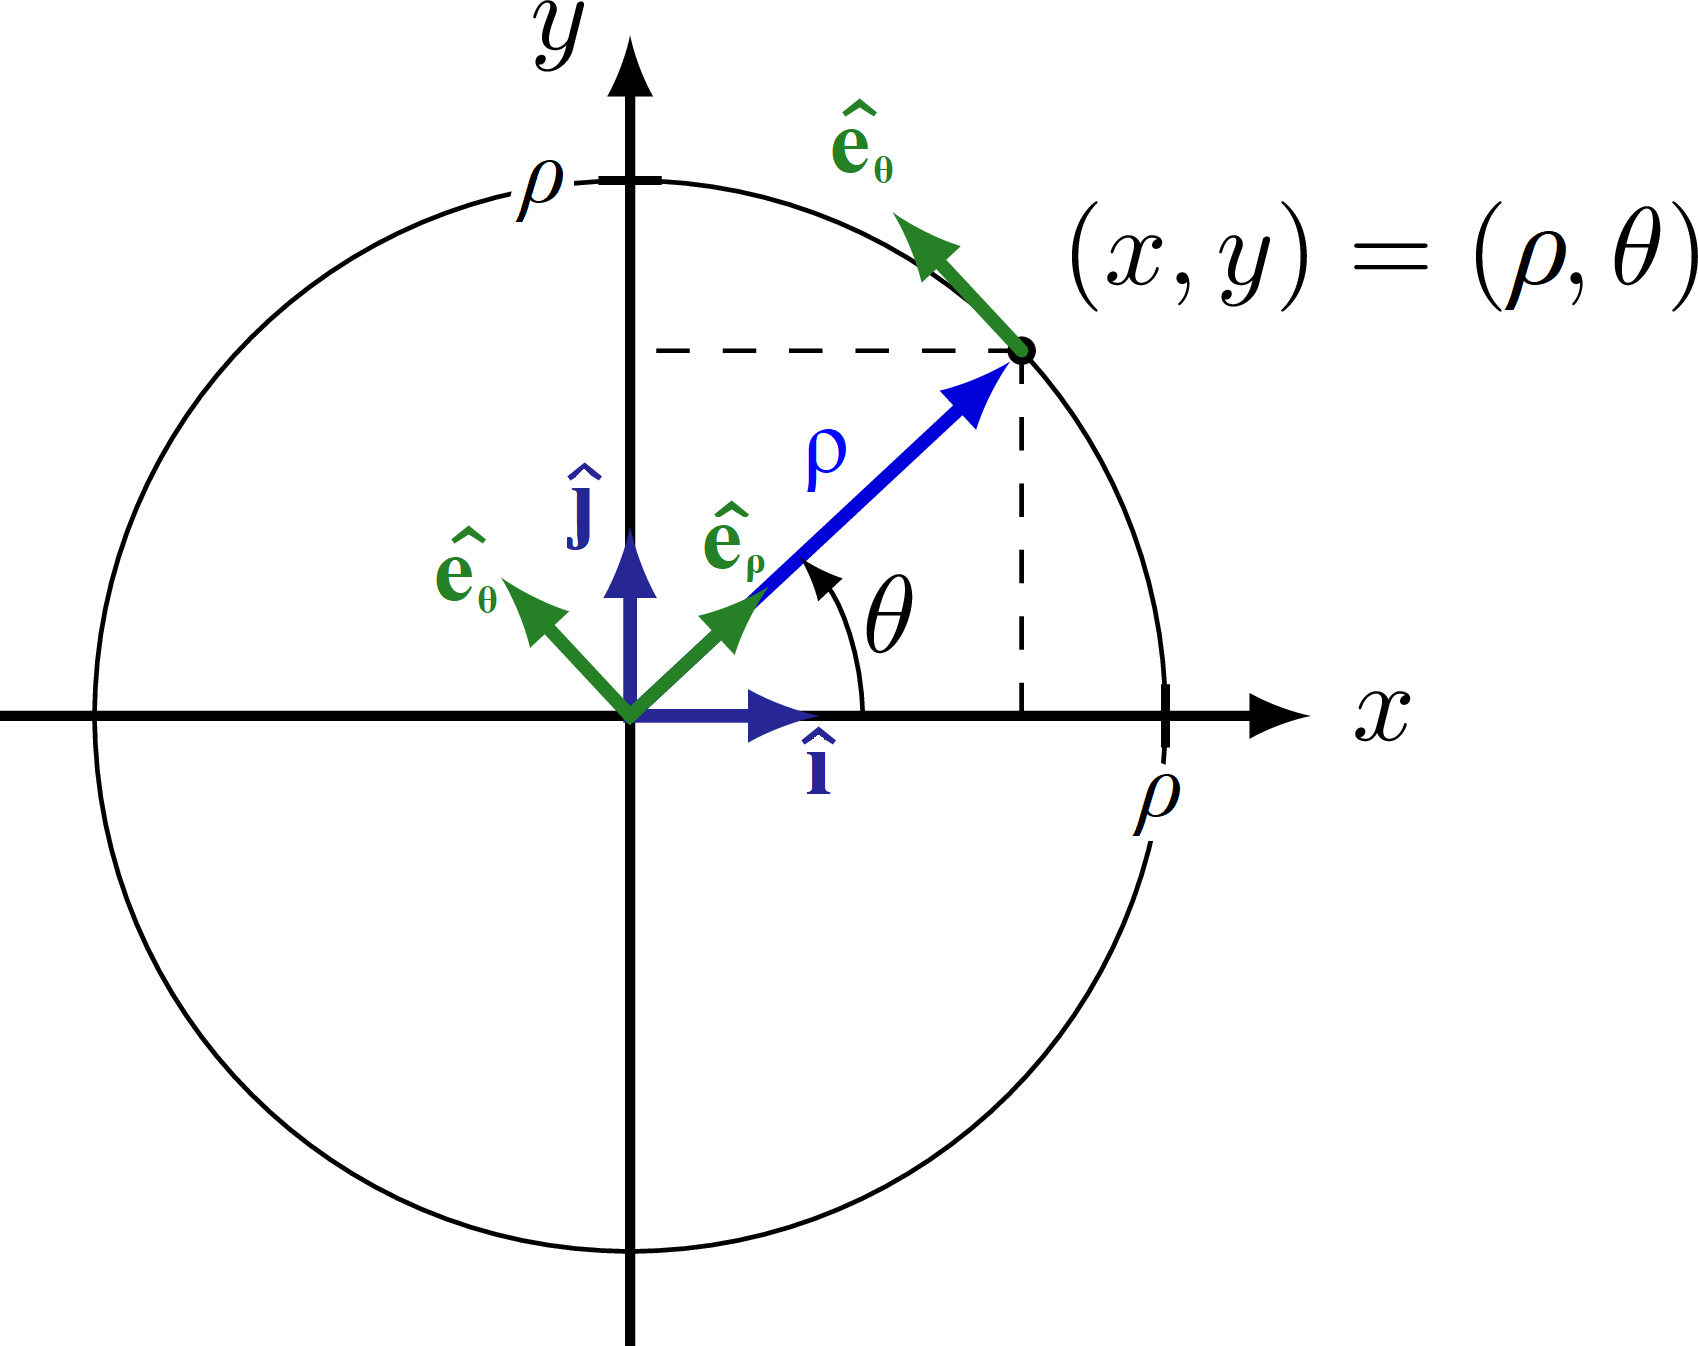
\includegraphics[scale = 0.18]{0}
\centering
\end{figure}

Para expresar la segunda ley de Newton en coordenadas polares, será necesario calcular el vector $\ddot{\vv{r}}$. Al derivar se obtiene
\[
\begin{aligned}[t]
\dot{\vv{r}} &= \dot{\rho}\hat{e_\rho}+\rho\dot{\hat{e_\rho}} = \dot{\rho}\hat{e_\rho}+\rho(-\dot{\theta}\sen{\theta} \, \hat{\imath}+\dot{\theta}\cos{\theta} \, \hat{\jmath}) = \dot{\rho}\hat{e_\rho}+\rho\dot{\theta}\hat{e_\theta} \\
\ddot{\vv{r}} &= \ddot{\rho}\hat{e_\rho}+\dot{\rho}\dot{\hat{e_\rho}}+\dot{\rho}\dot{\theta}\hat{e_\theta}+\rho\ddot{\theta}\hat{e_\theta}+\rho\dot{\theta}\dot{\hat{e_\theta}} = \ddot{\rho}\hat{e_\rho}+2\dot{\rho}\dot{\theta}\hat{e_\theta} +\rho\ddot{\theta}\hat{e_\theta}+\rho\dot{\theta}(-\dot{\theta}\cos{\theta} \, \hat{\imath}-\dot{\theta}\sen{\theta} \, \hat{\jmath}) = \\
&= \ddot{\rho}\hat{e_\rho}+2\dot{\rho}\dot{\theta}\hat{e_\theta}+\rho\ddot{\theta}\hat{e_\theta}-\rho\dot{\theta}^2\hat{e_\rho} = (\ddot{\rho}-\rho\dot{\theta}^2)\hat{e_\rho}+(2\dot{\rho}\dot{\theta}+\rho\ddot{\theta})\hat{e_\theta}
\end{aligned}
\]
Por tanto, la segunda ley de Newton quedaría como
\[m\ddot{\vv{r}} = \vv{F} \iff m(\ddot{\rho}-\rho\dot{\theta}^2)\hat{e_\rho}+m(2\dot{\rho}\dot{\theta}+\rho\ddot{\theta})\hat{e_\theta} = -\vv{\nabla}V\]
El término de la izquierda ya está expresado en coordenadas polares. Ahora hay que hacer lo propio con $-\vv{\nabla}V$. Como
\[-\vv{\nabla}V = -\frac{\partial V}{\partial x}\hat{\imath}-\frac{\partial V}{\partial y}\hat{\jmath} \tag{7}\]
entonces tenemos que expresar $\frac{\partial V}{\partial x},\hat{\imath},\frac{\partial V}{\partial y}$ y $\hat{\jmath}$ en función de $\rho$ y de $\theta$. Por un lado, de las ecuaciones (5) y (6) obtenemos un sistema de ecuaciones de la forma $AX = B$, donde
\[
A = \begin{pmatrix}
\cos{\theta} & \sen{\theta} \\
-\sen{\theta} & \cos{\theta}
\end{pmatrix}
\qquad
B = \begin{pmatrix}
\hat{e_\rho} \\
\hat{e_\theta}
\end{pmatrix}
\qquad
X = \begin{pmatrix}
\hat{\imath} \\
\hat{\jmath}
\end{pmatrix}
\]
Como $\det{(A)}=1 \neq 0$, entonces existe $A^{-1}$, y es precisamente
\[
A^{-1}=\frac{1}{\det{(A)}}\, \mathrm{adj} \, (A) = \begin{pmatrix}
    \cos\theta & -\sen\theta \\
    \sen\theta & \cos\theta
\end{pmatrix}
\]
luego
\[AX=B \iff X = A^{-1}B \iff 
\begin{pmatrix}
\hat{\imath} \\
\hat{\jmath}
\end{pmatrix}
=
\begin{pmatrix}
    \cos\theta & -\sen\theta \\
    \sen\theta & \cos\theta
\end{pmatrix}
\begin{pmatrix}
\hat{e_\rho} \\
\hat{e_\theta}
\end{pmatrix}
\]
de donde se deduce que
\[
\hat{\imath} = \cos\theta \, \hat{e_\rho}-\sen\theta \, \hat{e_\theta} \tag{8}
\]
\[
\hat{\jmath} = \sen\theta \, \hat{e_\rho}+\cos\theta \, \hat{e_\theta} \tag{9}
\]
Por otro lado, como la función $V$ depende de $x$ y de $y$ y estas, a su vez, dependen de $\rho$ y de $\theta$, entonces los valores que toma $V$ son de la forma $V(x(\rho,\theta),y(\rho,\theta))$. Por tanto, por la regla de la cadena,
\[
\begin{aligned}[t]
\frac{\partial V}{\partial \rho} &= \frac{\partial V}{\partial x}\frac{\partial x}{\partial \rho}+\frac{\partial V}{\partial y}\frac{\partial y}{\partial \rho} = \cos\theta \, \frac{\partial V}{\partial x}+\sen\theta \, \frac{\partial V}{\partial y} \\[5pt]
\frac{\partial V}{\partial \theta} &= \frac{\partial V}{\partial x}\frac{\partial x}{\partial \theta}+\frac{\partial V}{\partial y}\frac{\partial y}{\partial \theta} = -\rho \sen\theta \, \frac{\partial V}{\partial x}+\rho \cos\theta \, \frac{\partial V}{\partial y}
\end{aligned}
\]
De estas dos ecuaciones de obtiene otro sistema de la forma $AX=B$, donde
\[
A = \begin{pmatrix}
\cos{\theta} & \sen{\theta} \\
-\rho\sen{\theta} & \rho\cos{\theta}
\end{pmatrix}
\qquad
B = \begin{pmatrix}
\frac{\partial V}{\partial \rho} \\[5pt]
\frac{\partial V}{\partial \theta}
\end{pmatrix}
\qquad
X = \begin{pmatrix}
\frac{\partial V}{\partial x} \\[5pt]
\frac{\partial V}{\partial y}
\end{pmatrix}
\]
Como $\det{(A)}=\rho \neq 0$, entonces existe $A^{-1}$, y es precisamente
\[
A^{-1}=\frac{1}{\det{(A)}}\, \mathrm{adj} \, (A) = \frac{1}{\rho}\begin{pmatrix}
    \rho\cos\theta & -\sen\theta \\
    \rho\sen\theta & \cos\theta
\end{pmatrix}
\]
luego
\[AX=B \iff X = A^{-1}B \iff 
\begin{pmatrix}
\frac{\partial V}{\partial x} \\[5pt]
\frac{\partial V}{\partial y}
\end{pmatrix}
=
\begin{pmatrix}
    \cos\theta & -\frac{1}{\rho}\sen\theta \\[5pt]
    \sen\theta & \frac{1}{\rho}\cos\theta
\end{pmatrix}
\begin{pmatrix}
\frac{\partial V}{\partial \rho} \\[5pt]
\frac{\partial V}{\partial \theta}
\end{pmatrix}
\]
de donde se deduce que
\[
\frac{\partial V}{\partial x}=\cos\theta \, \frac{\partial V}{\partial \rho}-\frac{1}{\rho}\sen\theta \, \frac{\partial V}{\partial \theta} \tag{10}
\]
\[
\frac{\partial V}{\partial y}=\sen\theta \, \frac{\partial V}{\partial \rho}+\frac{1}{\rho}\cos\theta \, \frac{\partial V}{\partial \theta} \tag{11}
\]
Por tanto, sustituyendo en (7) las ecuaciones (8), (9), (10) y (11), quedaría
\small
\[
\begin{aligned}[t]
\vv{\nabla}V &= (\cos\theta \, \frac{\partial V}{\partial \rho}-\frac{1}{\rho}\sen\theta \, \frac{\partial V}{\partial \theta})(\cos\theta \, \hat{e_\rho}-\sen\theta \, \hat{e_\theta}) + (\sen\theta \, \frac{\partial V}{\partial \rho}+\frac{1}{\rho}\cos\theta \, \frac{\partial V}{\partial \theta})(\sen\theta \, \hat{e_\rho}+\cos\theta \, \hat{e_\theta}) \\
&= \cos^2\theta \, \frac{\partial V}{\partial \rho} \, \hat{e_\rho} - \cancel{\sen\theta \, \cos\theta \, \frac{\partial V}{\partial \rho} \hat{e_\theta}} - \cancel{\frac{1}{\rho} \, \sen\theta \, \cos\theta \, \frac{\partial V}{\partial \theta} \hat{e_\rho}}+\frac{1}{\rho} \, \sen^2 \theta \, \frac{\partial V}{\partial \theta} \hat{e_\theta} \, + \\
& \ \ \ \, \sen^2\theta \frac{\partial V}{\partial \rho} \hat{e_\rho}+\cancel{\sen\theta \, \cos\theta \frac{\partial V}{\partial \rho} \hat{e_\theta}}+\cancel{\frac{1}{\rho} \, \sen\theta \, \cos\theta \frac{\partial V}{\partial \theta} \hat{e_\rho}} + \frac{1}{\rho} \, \cos^2\theta \frac{\partial V}{\partial \theta} \, \hat{e_\theta} \\
&= \frac{\partial V}{\partial \rho}\hat{e_\rho}+\frac{1}{\rho}\frac{\partial V}{\partial \theta}\hat{e_\theta}
\end{aligned}
\]
\normalsize
Finalmente, regresando a la segunda ley de Newton,
\begin{align*}
m \ddot{\vv{r}} = -\vv{\nabla}V &\iff m(\ddot{\rho}-\rho\dot{\theta}^2)\hat{e_\rho}+m(2\dot{\rho}\dot{\theta}+\rho\ddot{\theta})\hat{e_\theta} = -\frac{\partial V}{\partial \rho}\hat{e_\rho}-\frac{1}{\rho}\frac{\partial V}{\partial \theta}\hat{e_\theta} \\
&\iff
\begin{cases}
\displaystyle m\ddot{\rho}-m\rho\dot{\theta}^2=-\frac{\partial V}{\partial \rho} \tag{12} \\
\\
\displaystyle m\rho^2\ddot{\theta}+2m\rho\dot{\rho}\dot{\theta} = -\frac{\partial V}{\partial \theta}
\end{cases}
\end{align*}

Esta es la expresión de la segunda ley de Newton en coordenadas polares. Partiendo de estas ecuaciones, vamos a obtener dos ecuaciones similares a (3) y (4) mediante un razonamiento análogo. La energía cinética del sistema es
\[T = \frac{1}{2}m|\dot{\vv{r}}|^2 = \frac{1}{2}m\dot{\rho}^2+\frac{1}{2}m\rho^2\dot{\theta}^2\]
Por tanto,
\[
\begin{aligned}[t]
 \frac{\partial T}{\partial \dot{\rho}} = m\dot{\rho} &\implies \frac{d}{dt}\biggl(\frac{\partial T}{\partial \dot{\rho}}\biggr) = \frac{d}{dt}m\dot{\rho} = m\ddot{\rho} \\
\frac{\partial T}{\partial \dot{\theta}} = m\rho^2\dot{\theta} &\implies \frac{d}{dt}\biggl(\frac{\partial T}{\partial \dot{\theta}}\biggr) = \frac{d}{dt}m\rho^2\dot{\theta} = 2m\rho\dot{\rho}\dot{\theta}+m\rho^2\ddot{\theta}
\end{aligned}
\]

\parindent=0pt
\vspace{2mm}
Sustituyendo en (12) estas ecuaciones, 
\[
\begin{aligned}[t]
\frac{d}{dt}\biggl(\frac{\partial T}{\partial \dot{\rho}}\biggr)-m\rho\dot{\theta}^2 &=-\frac{\partial V}{\partial \rho} \\
\frac{d}{dt}\biggl(\frac{\partial T}{\partial \dot{\theta}}\biggr) &=-\frac{\partial V}{\partial \theta}
\end{aligned}
\]

\vspace{2mm}
Al contrario de lo que ocurría antes de obtener las ecuaciones (3) y (4), ahora no siempre se tiene que $\frac{\partial T}{\partial \rho} = 0$ (aunque sí se sigue cumpliendo $\frac{\partial T}{\partial \theta} = 0$), ya que
\[\frac{\partial T}{\partial \rho} = m\rho\dot{\theta}^2\]
\parindent=1.5em
Por tanto, podemos escribir
\[
\begin{cases}
    \displaystyle \frac{d}{dt}\biggl(\frac{\partial T}{\partial \dot{\rho}}\biggr) - \frac{\partial T}{\partial \rho} - \frac{\partial (-V)}{\partial \rho} = 0 \\
    \\
    \displaystyle \frac{d}{dt}\biggl(\frac{\partial T}{\partial \dot{\theta}}\biggr) - \frac{\partial (-V)}{\partial \theta} = 0
\end{cases}
\]
O lo que es lo mismo, en términos del lagrangiano,
\[
\begin{cases}
    \displaystyle \frac{d}{dt}\biggl(\frac{\partial L}{\partial \dot{\rho}}\biggr) - \frac{\partial L}{\partial \rho} = 0 \\
    \\
    \displaystyle \frac{d}{dt}\biggl(\frac{\partial L}{\partial \dot{\theta}}\biggr) - \frac{\partial L}{\partial \theta} = 0
\end{cases}
\]
Estas ecuaciones son totalmente análogas a (3) y (4) sin más que cambiar $x$ e $y$ por $\rho$ y $\theta$.

\vspace{2mm}
En resumen, hemos visto que la expresión de la segunda ley de Newton en magnitudes vectoriales ($\vv{F} = m\ddot{\vv{r}}$) no se mantiene al cambiar el sistema de coordenadas. Sin embargo, las ecuaciones (3) y (4), que son totalmente equivalentes a esta ley en caso de que la fuerza $\vv{F}$ sea conservativa, sí que se mantienen al pasar de coordenadas cartesianas a coordenadas polares.



\section{Ecuación de Euler-Lagrange}

Dada una función $F \colon \R^3 \to \R$ diferenciable y dados $a,b,a',b' \in \R$ fijos con $a<b$, el problema fundamental del cálculo de variaciones consiste en buscar de entre el conjunto $M$ de todas las funciones $f \colon [a,b] \to \R$ suficientemente regulares y verificando  $f(a) = a'$ y $f(b) = b'$, cuáles de ellas consiguen maximizar o minimizar el número real
\[J(f) = \int_a^b F(f(t),f'(t),t)dt \tag{13}\]

Esto significa que si una función $f$ maximiza (resp. minimiza) el valor de $J(f)$, entonces cualquier función $\tilde{f} \colon [a,b] \to \R$ que resulte de variar ligeramente la función $f$ y que cumpla $\tilde{f}(a)=a'$ y $\tilde{f}(b)=b'$, debe verificar $J(\tilde{f}) < J(f)$ (resp. $J(\tilde{f}) > J(f)$). Esta \say{ligera variación de $f$} se puede expresar como
\[f(\varepsilon,t) = f(0,t)+\varepsilon \eta (t)\]
donde $\varepsilon > 0$ es próximo a 0 y $\eta$ es una función derivable que ha de verificar $\eta(a) =\eta(b)= 0$. Además, $f \colon \R^2 \to \R$ ahora representa a todas las funciones del conjunto $M$ mediante el parámetro $\varepsilon$, con la particularidad de que fijando $\varepsilon = 0$ se obtiene la función que da el valor extremo de $J$. En otras palabras, cualquier función de $M$ queda determinada por un $\varepsilon$ fijo, luego $(13)$ se puede escribir como
\[J(\varepsilon) = \int_a^b F(f(\varepsilon,t),\frac{\partial f}{\partial t}(\varepsilon,t),t)dt\]
Para simplificar la notación, se llamará $f' = \frac{\partial f}{\partial t}$ aunque $f$ no sea una función de una variable. Como los límites de integración son fijos, la derivación de $J$ afecta solo al integrando. Por tanto, por la regla de la cadena,
\[J'(\varepsilon) = \int_a^b \biggl(\frac{\partial F}{\partial f} \frac{\partial f}{\partial \varepsilon} + \frac{\partial F}{\partial f'} \frac{\partial f'}{\partial \varepsilon} \biggr)dt = \int_a^b \frac{\partial F}{\partial f} \eta(t) dt + \int_a^b \frac{\partial F}{\partial f'} \eta'(t) dt \tag{14}\]
Integrando por partes en el segundo sumando, se obtiene
\[\int_a^b \frac{\partial F}{\partial f'} \eta'(t) dt = \frac{\partial F}{\partial f'}\eta(t) \biggr]_a^b - \int_a^b \frac{d}{dt} \biggl(\frac{\partial F}{\partial f'} \biggr)\eta(t)dt = - \int_a^b \frac{d}{dt} \biggl(\frac{\partial F}{\partial f'} \biggr)\eta(t)dt\]
En la última igualdad se ha usado que $\eta(a)=\eta(b) = 0$. Sustituyendo en (14), quedaría 
\[J'(\varepsilon) = \int_a^b \biggl( \frac{\partial F}{\partial f}-\frac{d}{dt} \frac{\partial F}{\partial f'} \biggr)\eta(t)dt \tag{15}\]
Aunque no lo parezca, esta última integral depende de $\varepsilon$, pues $f$ y $f'$ dependen de $\varepsilon$. Además, se recuerda que para $\varepsilon = 0$, se verifica que $f(0,t)$ es la función que hace que el valor de $J$ sea máximo o mínimo, así que debe cumplirse $J'(0) = 0$. Esto significa que el integrando de la expresión
\[J'(0) = \int_a^b \biggl( \frac{\partial F}{\partial f}-\frac{d}{dt} \frac{\partial F}{\partial f'} \biggr)\eta(t)dt\]
debe ser nulo en el intervalo $(a,b)$. Ahora bien, como $\eta$ es una función cualquiera, pudiera ocurrir que no se anule en ningún punto de $(a,b)$, en cuyo caso tendría que verificarse

\setlength\fboxsep{0.3cm}
\setlength\fboxrule{1.5pt}
\[\boxed{\frac{\partial F}{\partial f}-\frac{d}{dt} \frac{\partial F}{\partial f'} = 0}\]
A esta ecuación se le conoce como \ul{ecuación de Euler-Lagrange}.

\begin{figure}[h]
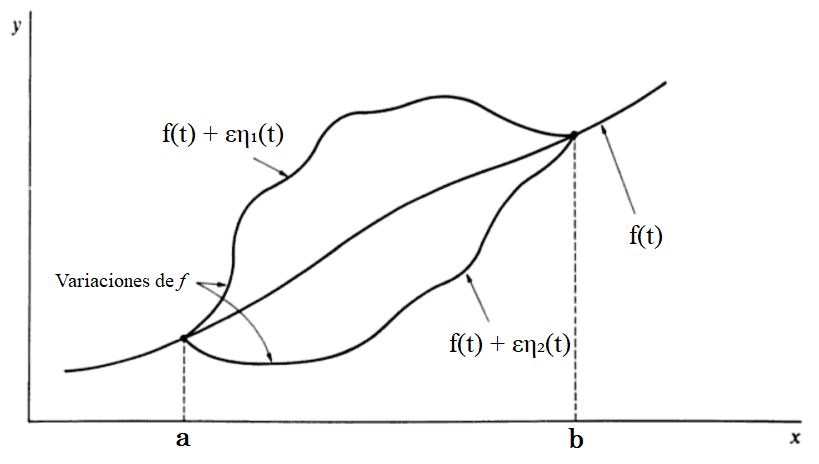
\includegraphics[scale = 0.5]{1.1_1}
\centering
\end{figure}

\vspace{2mm}
En un caso más general, supóngase que ahora $F$ está definida en $\R^n$ ($n \in \N$ impar mayor que $2$) y los valores que toma son de la forma $F(f_1(t),f'_1(t),f_2(t),f'_2(t),\mathellipsis,f_k(t),f'_k(t),t)$ para algún $k \in \N$, donde $f_i \colon [a,b] \to \R$ es suficientemente regular y verifica $f_i(a) = a', f_i(b) = b'$ para cualquier $i \in \{1,2,\mathellipsis,k\}$. En tal situación, se demuestra que la ecuación (15) ahora sería
\[J'(\varepsilon) = \int_a^b \sum_{i=1}^k \biggl( \frac{\partial F}{\partial f_i}-\frac{d}{dt} \frac{\partial F}{\partial f'_i} \biggr)\eta_i(t)dt \tag{16}\]
Por tanto, para cada $i \in \{1,2,\mathellipsis,k\}$, ha de cumplirse
\[\boxed{\frac{\partial F}{\partial f_i}-\frac{d}{dt} \frac{\partial F}{\partial f'_i} = 0}\]

\section{Ejemplos clásicos}

\begin{example}
Dados dos puntos del plano $A = (x_0,x_1)$ y $B = (x'_0,x'_1)$, vamos a hallar la distancia más corta entre dichos puntos, o lo que es lo mismo, hallar una curva $\alpha_y \colon [x_0,x'_0] \to \R^2$ que cumpla $\alpha_y(x_0) = A, \alpha_y(x'_0) = B$ y de forma que su longitud de curva sea mínima. Se puede suponer que la curva está definida por $\alpha_y(x) = (x,y(x))$ para cierta función $y \colon [x_0,x'_0] \to \R$ suficientemente regular, que ha de verificar $y(x_0) = x'_0, y(x_1) = x'_1$. La longitud de la curva se define como
\[L(y) = \int_{x_0}^{x'_0} ||\alpha'_y(x)|| \, dx = \int_{x_0}^{x'_0} \sqrt{1+y'(x)^2} \, dx\]
Por tanto, hay que aplicar la ecuación de Euler-Lagrange con $F \colon \R^3 \to \R$ definida por $F(y(x),y'(x),x)) = \sqrt{1+y'(x)^2}$:
\[
\begin{aligned}[t]
\frac{\partial F}{\partial y}-\frac{d}{dx} \frac{\partial F}{\partial y'} = 0 &\iff \frac{d}{dx} \frac{\partial F}{\partial y'} = 0 \iff \frac{\partial F}{\partial y'} = C \iff \frac{y'(x)}{\sqrt{1+y'(x)^2}} = C \\
&\implies y'(x)^2 = C^2(1+y'(x)^2) \iff y'(x)^2(1-C^2)= C^2 \\
&\implies y'(x) = \frac{C}{\sqrt{1-C^2}} \iff y(x) = \frac{C}{\sqrt{1-C^2}}x+B
\end{aligned}
\]
donde $B,C \in \R$ son constantes. Llamando $A = \frac{C}{\sqrt{1-C^2}}$, se tiene que $y(x) = Ax+B$, así que la curva en cuestión es, sorprendentemente, una recta.
\end{example}

\begin{example}[Braquistócrona]
Dados dos puntos del plano $A$ y $B$, se trata de construir un raíl sin rozamiento de forma que al dejar caer un vagón desde $A$, llegue a $B$ en el menor tiempo posible. Obviamente, será necesario que la coordenada en el eje $x$ de $A$ sea menor que la de $B$ y que la coordenada en el eje $y$ de $B$ sea menor que la de $A$.

\begin{figure}[h]
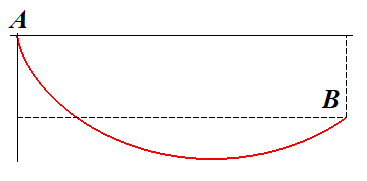
\includegraphics[scale = 0.5]{1.1_2}
\centering
\end{figure}

\vspace{2mm}
Calculemos la velocidad que lleva el vagón en cada punto $C$ de la trayectoria. Se considerará que la energía potencial vale cero en $A$. Como la única fuerza que actúa (la gravitatoria) es conservativa, entonces la energía mecánica permanece constante. Por tanto,
\[
\begin{aligned}[t]
T - V = 0 &\iff \frac{1}{2}mv^2 + \int_A^C \vv{F} \cdot d\vv{l} = 0 \\
&\iff \frac{1}{2}mv^2 - \int_A^C mg\hat{\jmath} \cdot dy\hat{\jmath} = 0 \\
&\iff \frac{1}{2}mv^2 - mgy = 0 \\
&\iff v = \sqrt{2gy} 
\end{aligned}
\]
donde $y$ es la coordenada en el eje $y$ del punto $C$. El tiempo que tarda el vagón en ir desde $A$ hasta $B$ se puede hallar como sigue:
\[
\begin{aligned}[t]
\Delta t &= t_B - t_A = r^{-1}(r_B) - r^{-1}(r_A) = \int_A^B (r^{-1})'(s) \, ds = \int_A^B \frac{1}{r'(r^{-1}(s))} \, ds = \int_A^B \frac{1}{r'(t)}dt \\ 
&= \int_A^B \frac{1}{v(t)}dt
\end{aligned}
\]

Se ha usado la regla de Barrow, el teorema de la derivada de la función inversa y el hecho de que $s$ no es más que la posición de una partícula en un instante dado, y por tanto $r(t) = s \implies t = r^{-1}(r(t)) = r^{-1}(s)$.

\vspace{2mm}
Se recuerda que la posición del vagón se puede expresar como función de la segunda coordenada, y por tanto los valores que toma son de la forma $(x(y),y)$. Para calcular la integral se hace el \textit{cambio de variable} (en Análisis se diría \textit{sustitución con $u$ invertible}) dado por \[t = r(y), \, dt = r'(y) \, dy = \sqrt{x'(y)^2+1} \, dy\] 
y utilizando que $v = \sqrt{2gy}$, quedaría
\[\Delta t = \int_A^B \frac{1}{\sqrt{2gy}}\sqrt{x'(y)^2+1} \, dy = \frac{1}{\sqrt{2g}} \int_A^B \frac{\sqrt{x'(y)^2+1}}{\sqrt{y}} \, dy\]

\noindent Tenemos que encontar una función $x$ de forma que la integral 
\[\int_A^B \frac{\sqrt{x'(y)^2+1}}{\sqrt{y}} \, dy = \int_A^B F(x,x',y) \, dy\]
tome el valor mínimo. Aplicando la ecuación de Euler-Lagrange,
\[\frac{\partial F}{\partial x} - \frac{d}{dy} \frac{\partial F}{\partial x'} = 0 \iff \frac{d}{dy}\frac{\partial F}{\partial x'} = 0\]
lo que significa que $\frac{\partial F}{\partial x'}$ es constante, luego
\[\frac{\partial F}{\partial x'} = \frac{x'}{\sqrt{y(x'^2+1)}} = k \implies \frac{x'^2}{y(x'^2+1)} = k^2\]
para cierto $k \in \R$. Podemos suponer que $k^2 = \frac{1}{2a}$ para cierto $a > 0$ adecuado, por lo que la ecuación quedaría
\[
\begin{aligned}[t]
\frac{x'^2}{y(x'^2+1)} = \frac{1}{2a} &\iff 2ax'^2 = yx'^2+y \iff x'^2(2a-y) = y \iff x' = \pm \frac{\sqrt{y}}{\sqrt{2a-y}} \\
&\iff x = \pm \int \frac{\sqrt{y}}{\sqrt{2a-y}}dy + c, \quad c \in \R
\end{aligned}
\]

Por la elección del sistema de referencia, tiene que ser $x \geq 0$ durante toda la trayectoria, así que se descarta el signo negativo. También se tomará $c = 0$ como constante de integración. Ahora calculamos la primitiva anterior mediante el cambio $y = a(1-\cos \theta); dy = a\sen\theta \, d\theta$:
\[
\begin{aligned}[t]
x &= \int \sqrt{\frac{a(1-\cos\theta)}{2a-a(1-\cos\theta)}}a\sen\theta \, d\theta = \int \sqrt{\frac{1-\cos\theta}{1+\cos\theta}}a\sen\theta \, d\theta \\
&= a \int \sqrt{\frac{(1-\cos\theta)\sen^2\theta}{1+\cos\theta}}d\theta = a \int(1-\cos\theta)d\theta = a(\theta - \sen\theta) + d, \quad d \in \R
\end{aligned}
\]

Como en el instante inicial se tiene que $x = 0$ y $y = 0$, entonces también es $\theta = 0$, así que hay que tomar $d = 0$. La solución del problema es 
\[x = a(\theta-\sen\theta)\]
\[y = a(1-\cos\theta)\]
\end{example}

\begin{example}
Se trata de encontrar el camino más corto entre dos puntos del espacio $P$ y $Q$. Al igual que en el primer ejemplo de esta sección, la distancia $s$ de este camino se puede expresar como la longitud de una curva dada por $\alpha(x) = (x,y(x),z(x))$ que en $P$ y $Q$ tome los valores adecuados, es decir,
\[
\begin{aligned}[t]
s &= \int_P^Q ||\alpha'(x)|| \, dx = \int_P^Q ||(1, y'(x), z'(x))|| \, dx = \int_P^Q \sqrt{1+y'(x)^2+z'(x)} \, dx
\end{aligned}
\]

El funcional de este problema está definido por $F(y,y',z,z',x) = \sqrt{1+y'^2+z'^2}$. Por las ecuaciones de Euler-Lagrange,

\[
\begin{aligned}[t]
\begin{cases}
\displaystyle \frac{\partial F}{\partial y}-\frac{d}{dx}\frac{\partial F}{\partial y'} = 0 \\
\\
\displaystyle \frac{\partial F}{\partial z}-\frac{d}{dx}\frac{\partial F}{\partial z'} = 0
\end{cases}
&\iff
\begin{cases}
\displaystyle \frac{d}{dx}\frac{\partial F}{\partial y'} = 0 \\
\\
\displaystyle \frac{d}{dx}\frac{\partial F}{\partial z'} = 0
\end{cases}
\iff
\begin{cases}
\displaystyle \frac{\partial F}{\partial y'} = a \\
\\
\displaystyle \frac{\partial F}{\partial z'} = b
\end{cases}
\iff
\begin{cases}
\displaystyle \frac{y'}{\sqrt{1+y'^2+z'^2}} = a \\
\\
\displaystyle \frac{z'}{\sqrt{1+y'^2+z'^2}} = b
\end{cases}
\\
&\implies
\begin{cases}
\displaystyle \frac{y'^2}{a^2} = 1+y'^2+z'^2 \\
\\
\displaystyle \frac{z'^2}{b^2} = 1+y'^2+z'^2
\end{cases}
\iff
\begin{cases}
(1-a^2)y'^2 -a^2z'^2= a^2 \\
\\
(1-b^2)z'^2 -b^2y'^2 = b^2
\end{cases}
\end{aligned}
\]
para ciertos $a,b \in \R$. Esto no es más que un sistema de ecuaciones de la forma $AX = B$, donde
\[A = \begin{pmatrix}
1-a^2 & -a^2 \\
-b^2 & 1-b^2
\end{pmatrix} \qquad X = 
\begin{pmatrix}
y'^2 \\
z'^2
\end{pmatrix} \qquad B = 
\begin{pmatrix}
a^2 \\
b^2
\end{pmatrix}
\]
A ningún físico le importaría que $a,b \in \R$ no fueran tales que $\mathrm{det}(A) = 1-b^2-a^2 \neq 0$. Por la regla de Cramer, la solución del sistema es
\[y'^2 = \frac{
\begin{vmatrix}
a^2 & -a^2 \\
b^2 & 1-b^2
\end{vmatrix}
}{1-b^2-a^2}
= \frac{a^2}{1-b^2-a^2} \implies y' = \pm \frac{a}{\sqrt{1-b^2-a^2}} = c_1, \quad c_1 \in \R\]
\[z'^2 = \frac{
\begin{vmatrix}
1-a^2 & a^2 \\
-b^2 & b^2
\end{vmatrix}
}{1-b^2-a^2}
= \frac{b^2}{1-b^2-a^2} \implies z' = \pm \frac{b}{\sqrt{1-b^2-a^2}} = c_2, \quad c_1 \in \R\]
y la solución del problema sería
\[y = c_1x+d_1, \qquad c_1,d_1 \in \R\]
\[z = c_2x+d_2, \qquad c_2,d_2 \in \R\]
que son las ecuaciones de dos planos (la ecuación de $y$ se verifica para cualquier valor de $z$ y la ecuación de $z$ se verifica para cualquier valor de $y$) cuya intersección es una recta que une los dos puntos iniciales, como era de esperar.

\end{example}

\section{Segunda forma de la ecuación de Euler-Lagrange}

El objetivo ahora es encontrar la segunda forma de la ecuación de Euler-Lagrange. La derivada de la función $F$ con respecto al tiempo es
\[\frac{dF}{dt} = f' \frac{\partial F}{\partial f} + f''\frac{\partial F}{\partial f'} + \frac{\partial F}{\partial t} \tag{17}\]
El término $f'' \frac{\partial F}{\partial f'}$ se puede escribir como
\[f'' \frac{\partial F}{\partial f'} = \frac{d}{dt}\biggl( f' \frac{\partial F}{\partial f'}\biggr) - f' \frac{d}{dt}\biggl( \frac{\partial F}{\partial f'}\biggr) \]
Sustituyendo en (17),
\[
\begin{aligned}[t]
\frac{dF}{dt} &= f' \frac{\partial F}{\partial f} + \frac{d}{dt}\biggl( f' \frac{\partial F}{\partial f'}\biggr) - f' \frac{d}{dt}\biggl( \frac{\partial F}{\partial f'}\biggr) + \frac{\partial F}{\partial t} = f'\biggl( \frac{\partial F}{\partial f} - \frac{d}{dt}\frac{\partial F}{\partial f'}\biggr)+\frac{d}{dt}\biggl( f' \frac{\partial F}{\partial f'}\biggr) + \frac{\partial F}{\partial t} \\
&= \frac{d}{dt}\biggl( f' \frac{\partial F}{\partial f'}\biggr) + \frac{\partial F}{\partial t}
\end{aligned}
\]
De esto se deduce que
\[\frac{d}{dt}\biggl( F - f'\frac{\partial F}{\partial f'} \biggr) = \frac{\partial F}{\partial t}\]
Por tanto, en los casos en que $F$ no dependa de $t$, se tiene que $\frac{\partial F}{\partial t} = 0$, así que existe una constante $k \in \R$ tal que

\setlength\fboxsep{0.3cm}
\setlength\fboxrule{1.5pt}
\[\boxed{F - f'\frac{\partial F}{\partial f'} = k}\]
Esta es la \ul{segunda forma de la ecuación de Euler-Lagrange}.

\section{Condiciones auxiliares}

En la práctica, además de las condiciones tratadas anteriormente, se impondrán otro tipo de requisitos, como que una curva satisfaga la ecuación de una determinada superficie a la hora de encontrar la distancia más corta entre dos puntos. Esto es lo que sucede en el cálculo de la geodésica del cilindro, la esfera o el cono, por ejemplo.

\vspace{2mm}
A continuación se estudiará el caso particular en que las condiciones auxiliares vienen dadas por una ecuación de la forma
\[g(f_1,f_2,t) = 0 \tag{18}\]
para cierta función $g$ suficientemente regular. Además, se supondrá que la función $F$ que se presenta en el integrando del funcional es de la forma $F(f_1,f_2,f'_1,f'_2,t)$. Uitlizando la ecuación $(16)$ en el caso $k = 2$, el funcional $J$ se puede expresar como
\[J'(\varepsilon) = \int_a^b \biggl[ \biggl( \frac{\partial F}{\partial f_1}-\frac{d}{dt} \frac{\partial F}{\partial f'_1} \biggr) \eta_1(t) + \biggl( \frac{\partial F}{\partial f_2}-\frac{d}{dt} \frac{\partial F}{\partial f'_2} \biggr) \eta_2(t) \biggr]dt\]
Recuérdese que para $i = 1,2$, la función $\eta_i$ verifica $f_i(\varepsilon,t) = f_i(0,t) + \varepsilon \eta_i(t)$.  Derivando respecto de $\varepsilon$, se tiene que 
\[\frac{\partial f_i}{\partial \varepsilon} = \eta_i(t)\]
Sustituyendo, se obtiene
\[J'(\varepsilon) = \int_a^b \biggl[ \biggl( \frac{\partial F}{\partial f_1}-\frac{d}{dt} \frac{\partial F}{\partial f'_1} \biggr) \frac{\partial f_1}{\partial \varepsilon} + \biggl( \frac{\partial F}{\partial f_2}-\frac{d}{dt} \frac{\partial F}{\partial f'_2} \biggr) \frac{\partial f_2}{\partial \varepsilon} \biggr]dt \tag{19}\]
Recuérdese que la función $g$ depende de $\varepsilon$, pues $f_1$ y $f_2$ dependen de $\varepsilon$. Por tanto, derivando $g$ respecto de $\varepsilon$ e igualando a $0$,
\[\frac{\partial g}{\partial \varepsilon} = 0 \iff \frac{\partial g}{\partial f_1}\frac{\partial f_1}{\partial \varepsilon} + \frac{\partial g}{\partial f_2}\frac{\partial f_2}{\partial \varepsilon} = 0 \iff \frac{\partial f_2}{\partial \varepsilon} = -\frac{\partial g}{\partial f_1}\frac{\partial f_1}{\partial \varepsilon} \biggl( \frac{\partial g}{\partial f_2} \biggr)^{-1}\]
Pudiera ocurrir que el término $\frac{\partial g}{\partial f_2}$ fuese nulo y esta última expresión no tenga sentido, pero un físico de categoría haría la vista gorda y tiraría hacia delante. Sustituyendo ahora en (19), quedaría
\[
\begin{aligned}[t]
J'(\varepsilon) &= \int_a^b \biggl[ \biggl( \frac{\partial F}{\partial f_1}-\frac{d}{dt} \frac{\partial F}{\partial f'_1} \biggr)\frac{\partial f_1}{\partial \varepsilon} - \biggl( \frac{\partial F}{\partial f_2}-\frac{d}{dt} \frac{\partial F}{\partial f'_2} \biggr) \biggl(\frac{\partial g}{\partial f_1}\frac{\partial f_1}{\partial \varepsilon} \biggr) \biggl( \frac{\partial g}{\partial f_2} \biggr)^{-1} \biggr]dt \\
&= \int_a^b \biggl[ \biggl( \frac{\partial F}{\partial f_1}-\frac{d}{dt} \frac{\partial F}{\partial f'_1} \biggr) - \biggl( \frac{\partial F}{\partial f_2}-\frac{d}{dt} \frac{\partial F}{\partial f'_2} \biggr) \biggl(\frac{\partial g}{\partial f_1} \biggr) \biggl( \frac{\partial g}{\partial f_2} \biggr)^{-1} \biggr]\frac{\partial f_1}{\partial \varepsilon} \, dt
\end{aligned}
\]
Imponiendo la condición de extremo (que es $J'(0) = 0$), ha de ocurrir que la función del integrando anterior sea nula. Ahora bien, como la función $\frac{\partial f_1}{\partial \varepsilon}$ podría no anularse en algún punto, entonces debe cumplirse
\[\biggl( \frac{\partial F}{\partial f_1}-\frac{d}{dt} \frac{\partial F}{\partial f'_1} \biggr) - \biggl( \frac{\partial F}{\partial f_2}-\frac{d}{dt} \frac{\partial F}{\partial f'_2} \biggr) \biggl(\frac{\partial g}{\partial f_1} \biggr) \biggl( \frac{\partial g}{\partial f_2} \biggr)^{-1} = 0\]
o lo que es lo mismo, multiplicando por $(\frac{\partial g}{\partial f_1})^{-1}$,
\[\biggl( \frac{\partial F}{\partial f_1}-\frac{d}{dt} \frac{\partial F}{\partial f'_1} \biggr)\biggl(\frac{\partial g}{\partial f_1} \biggr)^{-1} = \biggl( \frac{\partial F}{\partial f_2}-\frac{d}{dt} \frac{\partial F}{\partial f'_2} \biggr) \biggl( \frac{\partial g}{\partial f_2} \biggr)^{-1}\]
Ambos miembros de tal igualdad son funciones que dependen de $t$, y por tanto, se puede considerar una función $\lambda$ que haya de verificar
\[
\begin{cases}
\displaystyle -\lambda(t) = \biggl( \frac{\partial F}{\partial f_1}-\frac{d}{dt} \frac{\partial F}{\partial f'_1} \biggr)\biggl(\frac{\partial g}{\partial f_1} \biggr)^{-1} \\[0.5cm]
\displaystyle -\lambda(t) = \biggl( \frac{\partial F}{\partial f_2}-\frac{d}{dt} \frac{\partial F}{\partial f'_2} \biggr) \biggl( \frac{\partial g}{\partial f_2} \biggr)^{-1}
\end{cases} \!\!\!\! \iff \begin{cases}
\displaystyle \biggl( \frac{\partial F}{\partial f_1}-\frac{d}{dt} \frac{\partial F}{\partial f'_1} \biggr) +\lambda(t)\biggl(\frac{\partial g}{\partial f_1} \biggr) =0\\[0.5cm]
\displaystyle\biggl( \frac{\partial F}{\partial f_2}-\frac{d}{dt} \frac{\partial F}{\partial f'_2} \biggr) +\lambda(t)\biggl( \frac{\partial g}{\partial f_2} \biggr) =0
\end{cases} \tag{20}
\]

La resolución del problema consistirá entonces en determinar $f_1,f_2$ y $\lambda$. Para ello, se disponen de las dos ecuaciones (20) y de la ecuación de ligadura (18), que son suficientes para poder encontrar la deseada solución.

\vspace{2mm}
En un caso más general, si se tienen $n$ funciones $f_1,f_2,\mathellipsis,f_n$ y $m$ ecuaciones de ligadura de la forma
\[g_k(f_j,t)=0, \qquad j = 1,\mathellipsis,n, k = 1,\mathellipsis,m\]
entonces las ecuaciones serán
\[\boxed{\frac{\partial F}{\partial f_j}-\frac{d}{dt}\frac{\partial F}{\partial f_j'} + \sum_k \lambda_k(t)\frac{\partial g_k}{\partial f_j} = 0}\]
Las funciones $\lambda_k$ se denominan \ul{multiplicadores de Lagrange}.

\chapter{Mecánica lagrangiana}

\section{Principio de Hamilton}

\noindent \textbf{Principio de Hamilton.} \textit{De todas las trayectorias posibles que puede seguir un sistema dinámico para desplazarse de un punto a otro durante un determinado intervalo de tiempo $[t_1,t_2]$, la trayectoria seguida es aquella que hace que la integral}
\[\int_{t_1}^{t_2}(T-V) \, dt = \int_{t_1}^{t_2} L \, dt \tag{1}\]
\textit{sea mínima.}

\vspace{2mm}
Fijado un sistema de coordenadas, la energía cinética de una partícula depende solo de la velocidad $\dot{x}_i$, mientras que, en caso de solo actuar fuerzas conservativas, la energía potencial solo depende de la posición $x_i$. Es por ello que el lagrangiano $L = T-V$ depende de la velocidad $\dot{x}_i$, de la posición $x_i$ y del tiempo $t$, de forma que $(1)$ se puede expresar como
\[\int_{t_1}^{t_2} L(\dot{x}_i, x_i, t) \, dt\]
e invocando las ecuaciones de Euler-Lagrange se obtiene
\[\frac{d}{dt}\frac{\partial L}{\partial \dot{x}_i} - \frac{\partial L}{\partial x_i} = 0\]
lo que proporciona unas ecuaciones idénticas a las que se vieron en la sección 1.1.

\begin{example}

Se van a hallar las ya conocidas ecuaciones del movimiento de una partícula pegada a un muelle:

\begin{figure}[h]
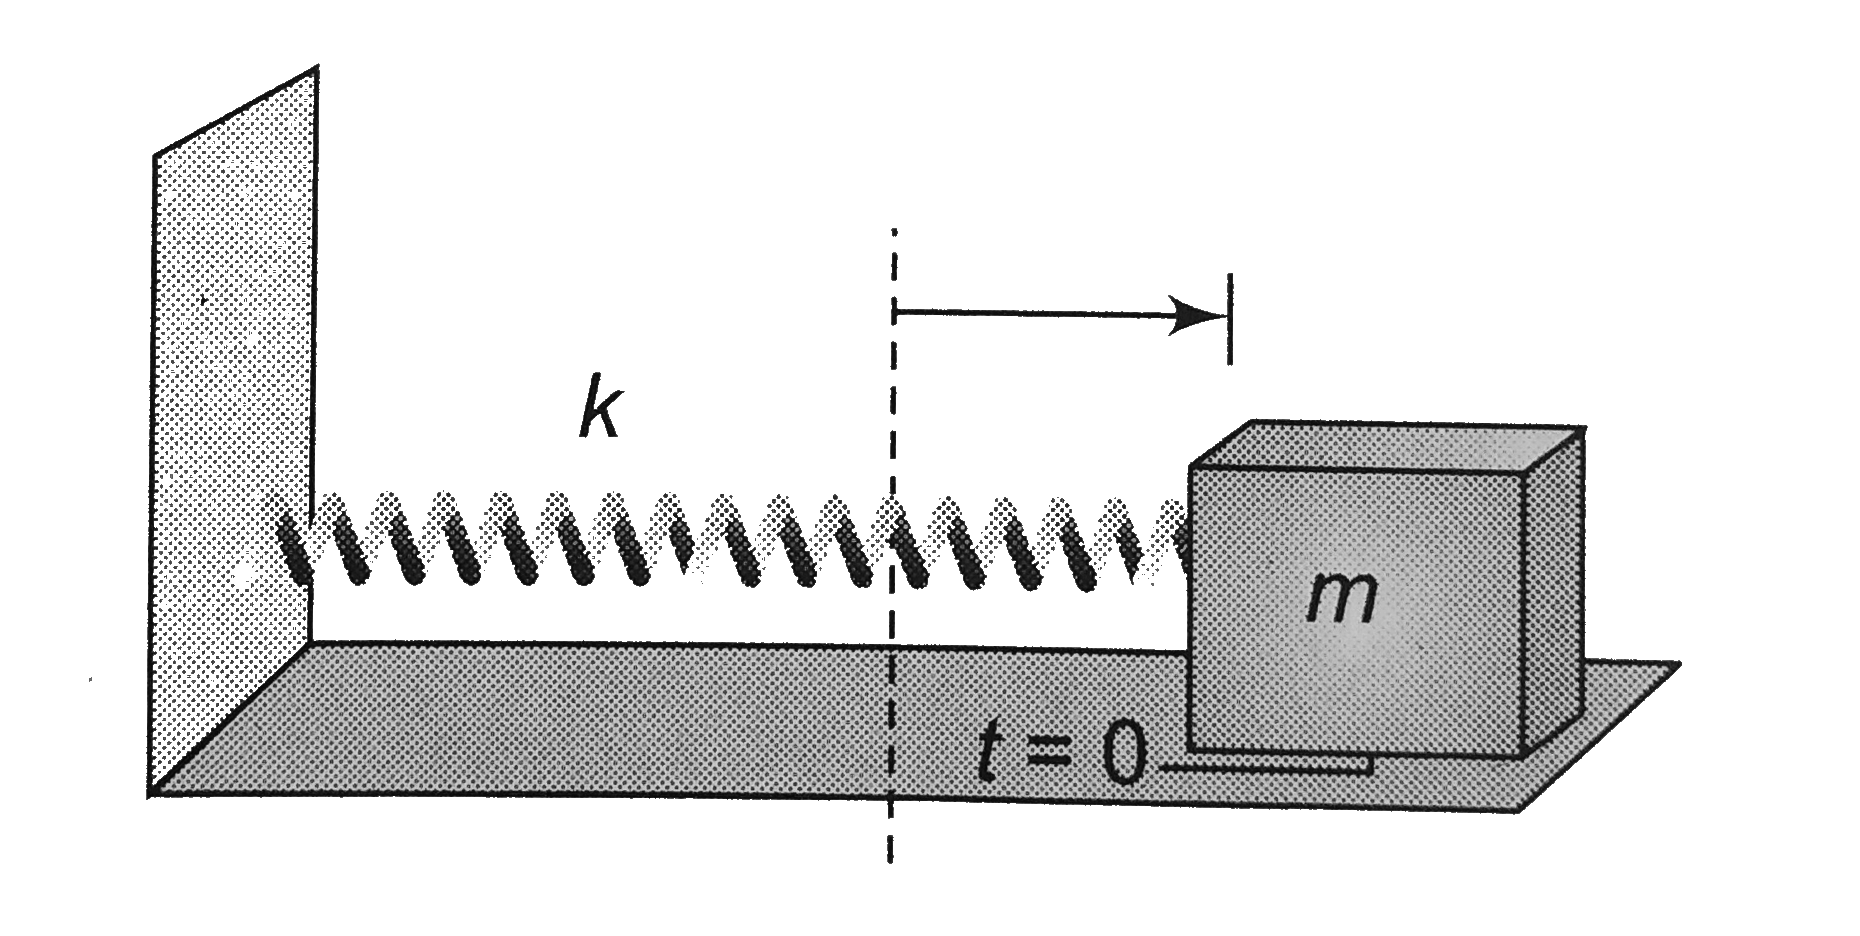
\includegraphics[scale = 0.075]{2.1_1}
\centering
\end{figure}

\noindent El lagrangiano del sistema es
\[L = T- V= \frac{1}{2}m\dot{x}^2 - \frac{1}{2}kx^2\]
Por tanto,
\[
\frac{d}{dt}\frac{\partial L}{\partial \dot{x}} - \frac{\partial L}{\partial x} = 0 \iff m \ddot{x} + kx = 0 \iff \ddot{x} + \frac{k}{m}x = 0 \iff \ddot{x}+\omega^2 x = 0
\]

Se trata de una ecuación diferencial lineal de segundo orden homogénea con coeficientes constantes, cuya ecuación característica es $\lambda^2+\omega^2 = 0$, que tiene como solución $\lambda = \omega i$. Por tanto, la solución general de la ecuación diferencial es
\[x(t) = c_1 \cos(\omega t) + c_2 \sen(\omega t), \qquad c_1,c_2 \in \R\]

Suponiendo $x(0) = 0$, entonces tiene que ser $c_1 = 0$. Además, en el instante $\frac{T}{4}$ ($T$ es el periodo), la posición del cuerpo es la amplitud $A$, luego 
\[A = x\biggr(\frac{T}{2}\biggr) = c_2 \sen\biggl(\frac{2\pi}{T}\frac{T}{4}\biggr) = c_2 \]
de forma que la ecuación es $x(t) = A \sen(\omega t)$. Si en el instante $t = 0$ el cuerpo no se encuentra en la posición de equilibrio, sino que tiene un \textit{desfase} $\varphi_0$, entonces la ecuación anterior es la sonada ecuación del movimiento armónico simple, $x(t) = A \sen(\omega t + \varphi_0)$, ó bien $x(t) = A \cos(\omega t + \varphi_0)$, dependiendo de la posición inicial.

\end{example}

\begin{example}

Se hallará ahora la ecuación del movimento en una caída libre. El lagrangiano del sistema es
\[L = \frac{1}{2}m\dot{y}^2-mgy\]
Por tanto,
\[
\begin{aligned}[t]
\frac{d}{dt}\frac{\partial L}{\partial \dot{y}} - \frac{\partial L}{\partial y} = 0 &\iff m \ddot{y} +mg = 0 \iff \ddot{y} = -g \iff \dot{y} = -gt + c_1 \\
&\iff y = -\frac{1}{2}gt^2+c_1t+c_2, \qquad c_1, c_2 \in \R
\end{aligned}
\]
Llamando $\dot{y}(0) = v_0, y(0) = y_0$, se tiene que
\[y(t) = -\frac{1}{2}gt^2+v_0t+y_0\]
\end{example}

\begin{example}
Ahora el tiro parabólico. El lagrangiano sería
\[L = \frac{1}{2}m\dot{x}^2+\frac{1}{2}m\dot{y}^2-mgy\]
En este caso hay dos ecuaciones de Euler-Lagrange. La primera sería
\[
\begin{aligned}[t]
\frac{d}{dt}\frac{\partial L}{\partial \dot{x}} - \frac{\partial L}{\partial x} = 0 \iff m \ddot{x} = 0 \iff \ddot{x} = 0 \iff \dot{x} = c_1 \iff x = c_1t + c_2, \qquad c_1, c_2 \in \R
\end{aligned}
\]
y como $v_0 = \dot{x}(0) = c_1$ y $x_0 = x(0) = c_2$, entonces
\[x(t) = v_0t+x_0\]
La otra ecuación de Euler-Lagrange es
\[
\begin{aligned}[t]
\frac{d}{dt}\frac{\partial L}{\partial \dot{x}} - \frac{\partial L}{\partial x} = 0 \iff m \ddot{y}+mg = 0 \iff \ddot{y} = -g
\end{aligned}
\]
En el ejemplo anterior ya se vio que
\[y(t) = -\frac{1}{2}gt^2+v_0t+y_0\]

Las dos ecuaciones obtenidas describen por completo el movimiento del proyectil en un tiro parabólico.
\end{example}

\section{Coordenadas generalizadas}

En esta sección se tratará de aprovechar el hecho de que el lagrangiano de un sistema permanece invariante frente a cambios de coordenadas. 

\vspace{2mm}
Considérese un sistema mecánico compuesto por $N$ partículas. Se tienen entonces $N$ vectores de posición con $3$ coordenadas cada uno, así que para describir las posiciones de todas las partículas deberán darse $3N$ cantidades. 

\vspace{2mm}
En algunos casos existirán ecuaciones de ligadura que relacionen algunas de estas $3N$ coordenadas con otras, de forma que las $3N$ coordenadas no serán independientes entre sí. Ocurre que si el sistema cuenta con $M$ ecuaciones de ligadura, el número de coordenadas independientes es $3N-M$. Se dirá en esta situación que el sistema posee $S = 3N-M$ \ul{grados de libertad}.

\vspace{2mm}
De esta manera, el estado del sistema quedará definido por $S$ parámetros, llámense $q_1,q_2,\mathellipsis,q_S$. Estas misteriosas cantidades se conocen como \ul{coordenadas generalizadas}. De las derivadas respecto al tiempo de las coordenadas generalizadas $\dot{q}_1,\dot{q}_2,\mathellipsis,\dot{q}_s$ se dirá que son las \ul{velocidades generalizadas}.

\vspace{2mm}
Que el sistema esté determinado por las $S$ coordenadas generalizadas quiere decir que el estado del mismo quedará descrito por un punto de un espacio de dimensión $S$, al que se llamará \ul{espacio de configuraciones}. Además, las $3N$ coordenadas cartesianas se podrán expresar en función de estas coordenadas generalizadas. Esto se escribirá como
\[x_i = x_i(q_1,q_2,\mathellipsis,q_S,t) = x_i(q_j,t), \qquad i = 1,\mathellipsis,3N, \, j = 1,\mathellipsis,S\]
En cuanto a las velocidades, se escribirá
\[\dot{x}_i = \dot{x}_i(q_j,\dot{q}_j,t), \qquad i = 1,\mathellipsis,3N, \, j = 1,\mathellipsis,S\]

Utilizando todo este embrollo de las coordenadas generalizadas, el principio de Hamilton puede ser reformulado como sigue:

\noindent \textbf{Principio de Hamilton.} \textit{De todas las trayectorias posibles que puede seguir un sistema dinámico para desplazarse de un punto a otro del espacio de configuraciones durante un intervalo de tiempo $[t_1,t_2]$ determinado, la trayectoria seguida es aquella que hace que las integrales}
\[\int_{t_1}^{t_2} L(q_i,\dot{q}_i,t) \, dt, \qquad i = 1,\mathellipsis,S\]
\textit{sean mínimas.}

\vspace{2mm}
Así, las $S$ ecuaciones de Euler-Lagrange que se usarán para describir el sistema serían en este caso

\[\boxed{\frac{d}{dt}\frac{\partial L}{\partial \dot{q}_i} - \frac{\partial L}{\partial q_i} = 0, \qquad i = 1,\mathellipsis,S}\]

Las ecuaciones anteriores proporcionan $S$ ecuaciones diferenciales de segundo orden. Para obtener soluciones únicas, será necesario que se proporcionen $2S$ condiciones iniciales (una para $q_i$ y otra para $\dot{q}_i$, para todo $i = 1,\mathellipsis,S$).

\vspace{2mm}
En cuanto a las $M$ ligaduras, se dijo al principio de la sección que en cada instante de tiempo deben relacionar las coordenadas del sistema. Si las ligaduras no dependen de la velocidad, es decir, si se pueden expresar de la forma
\[ G_k(q_i, t) = 0, \qquad k = 1,\mathellipsis,M, i = 1,\mathellipsis,S\]
se dirá que son ligaduras \ul{holónomas}. En caso contrario, si se tiene
\[G_k(q_i,\dot{q}_i, t) = 0, \qquad k = 1,\mathellipsis,M, i = 1,\mathellipsis,S\]
 las ligaduras se dirán \ul{no holónomas}. 
 
 \vspace{2mm}
 Por otro lado, supóngase que una ecuación de ligadura $h(q_j,\dot{q}_j,t) = 0$ se puede expresar de la forma 
\[\sum_j\frac{\partial g}{\partial q_j} \dot{q_j} + \frac{\partial g}{\partial t} = 0\]
donde $g(q_j,t), \, j = 1,\mathellipsis,S$ es una cierta función suficientemente regular. Lo anterior también se puede escribir como
\[\frac{dg}{dt} = 0\]
así que $g$ es una función constante. La condición $g(q_j,t) = k$ no es más que una ligadura holónoma. Es por ello que una ligadura de este estilo se llama \ul{ligadura cuasiholónoma}.

\begin{example}[Péndulo simple] El panorama se describe en la figura de la página siguiente. La primera restricción es que el péndulo se mueve en el plano, de forma que $z = 0$; la segunda es que en cada punto $(x,y)$ se verifica $x^2+y^2 = l^2$, donde $l$ es constante. Por tanto, $M = 2$, y como solo hay una partícula, es $N = 1$, así que se tiene $S = 3 \cdot 1 - 2 = 1$ grado de libertad. Por otro lado, como $x = \pm \sqrt{l^2-y^2}$, entonces
\[T = \frac{1}{2}m(\dot{x}^2+\dot{y}^2) = \frac{1}{2}m\biggl(\biggl(\frac{y\dot{y}}{\sqrt{l^2-y^2}}\biggr)^2+\dot{y}^2\biggr) = \frac{ml^2\dot{y}^2}{2(l^2-y^2)}\]
luego el lagrangiano del sistema es
\[L = \frac{ml^2\dot{y}^2}{2(l^2-y^2)} + mgy\]

Nótese que en nada influye la elección del signo positivo o negativo de $x$. La única ecuación de Euler-Lagrange sería
\[
\begin{aligned}[t]
\frac{d}{dt}\frac{\partial L}{\partial \dot{y}}-\frac{\partial L}{\partial y} = 0 &\iff \frac{d}{dt}\biggl(\frac{ml^2\dot{y}}{l^2-y^2}\biggr)-\biggl(\frac{ml^2\dot{y}^2y}{(l^2-y^2)^2}+mg \biggr) = 0 \\
&\iff \frac{ml^2\ddot{y}}{l^2-y^2}+\frac{2ml^2\dot{y}^2y}{(l^2-y^2)^2} -\frac{ml^2\dot{y}^2y}{(l^2-y^2)^2}-mg = 0 \\
&\iff \frac{l^2\ddot{y}}{l^2-y^2}+\frac{l^2\dot{y}^2y}{(l^2-y^2)^2}-g=0 \\
&\iff \ddot{y}+\frac{\dot{y}^2y}{l^2-y^2}-\frac{(l^2-y^2)g}{l^2}=0 \\
&\iff \ddot{y}+\frac{\dot{y}^2y}{l^2-y^2}+\frac{y^2g}{l^2}=g
\end{aligned}
\]
ecuación que describe por completo la posición de la partícula en cada instante de tiempo.

\begin{figure}[h]
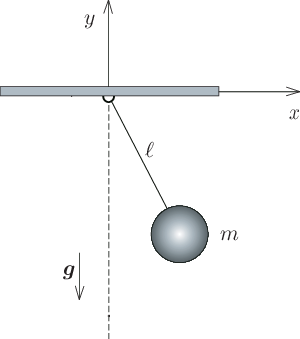
\includegraphics[scale = 0.6]{2.2_1}
\centering
\end{figure}

\vspace{2mm}
En lugar de expresar $x$ en función de $y$ y hacer los cálculos pertinentes, se va a proceder ahora a la inversa con la esperanza de obtener una ecuación más agradable a la vista. Teniendo en cuenta que en el sistema de referencia elegido es siempre $y \geq 0$, se tiene entonces
\[y = \sqrt{l^2-x^2} \qquad \dot{y} = -\frac{x\dot{x}}{\sqrt{l^2-x^2}}\]
Por tanto,
\[T = \frac{1}{2}m(\dot{x}^2+\dot{y}^2) = \frac{1}{2}m\biggl(\dot{x}^2+\frac{x^2\dot{x}^2}{l^2-x^2}  \biggr)= \frac{ml^2\dot{x}^2}{2(l^2-x^2)}\]
y el lagrangiano en este caso es
\[L = \frac{ml^2\dot{x}^2}{2(l^2-x^2)}+mg\sqrt{l^2-x^2} \]
Aplicando de nuevo la ecuación de Euler-Lagrange,
\[
\begin{aligned}[t]
\frac{d}{dt}\frac{\partial L}{\partial \dot{x}}-\frac{\partial L}{\partial x} = 0 &\iff \frac{d}{dt}\biggl(\frac{ml^2\dot{x}}{l^2-x^2}\biggr)-\biggl(\frac{ml^2\dot{x}^2x}{(l^2-x^2)^2}-\frac{mgx}{\sqrt{l^2-x^2}} \biggr) = 0 \\
&\iff \frac{ml^2\ddot{x}}{l^2-x^2}+\frac{2ml^2\dot{x}^2x}{(l^2-x^2)^2}-\frac{ml^2\dot{x}^2x}{(l^2-x^2)^2}+\frac{mgx}{\sqrt{l^2-x^2}} = 0 \\
&\iff \frac{ml^2\ddot{x}}{l^2-x^2}+\frac{ml^2\dot{x}^2x}{(l^2-x^2)^2}+\frac{mgx}{\sqrt{l^2-x^2}}=0 \\
&\iff \ddot{x} + \frac{\dot{x}^2x}{l^2-x^2} + \frac{gx\sqrt{l^2-x^2}}{l^2} = 0 \\
&\iff \ddot{x}+\frac{x}{l^2}\frac{\dot{x}^2}{1-\frac{x^2}{l^2}}+\frac{g}{l}x\sqrt{1-\frac{x^2}{l^2}}=0
\end{aligned}
\]
En el péndulo simple se puede considerar que $x$ es pequeño con respecto a $l$, de forma que $\frac{x}{l^2} \approx 0$ y $\frac{x^2}{l^2} \approx 0$. La expresión final sería
\[\ddot{x}+\frac{g}{l}x=0\]
ecuación que debe resultar más familiar que la otra que se obtuvo.

\vspace{2mm}
Si se decidiera resolver el problema mediante coordenadas polares, las dos restricciones serían $z = 0$ y $\rho = l$, donde $l$ es constante. Suponiendo que $\theta$ es siempre menor que $10^\circ$, la ecuación que se obtendría sería, expresando $\rho$ en función de $\theta$,
\[\ddot{\theta}+\frac{g}{l}\theta = 0\]
\end{example}

\section{Multiplicadores de Lagrange}

Se estudiará el caso particular de un sistema en que se tienen $M$ ecuaciones de ligadura holónomas, es decir, ecuaciones de la forma
\[g_k(q_j,t) = 0, \qquad j = 1,\mathellipsis,S, \ k = 1,\mathellipsis,M\]
Si se recuerda la última ecuación del primer tema y se aplica para $F = L$ (en este caso la integral que se quiere minimizar es la del principio de Hamilton), para cada $j$ deberá cumplirse
\[\frac{\partial L}{\partial q_j} - \frac{d}{dt}\frac{\partial L}{\partial \dot{q}_j} + \sum_k\lambda_k(t)\frac{\partial g_k}{\partial q_j} = 0 \tag{2}\]
El significado físico de los multiplicadores de Lagrange es que las funciones
\[\boxed{R_{k,j} = \lambda_k(t) \frac{\partial g_k}{\partial q_j}} \qquad j = 1,\mathellipsis,S, \ k = 1,\mathellipsis,M\]
son las componentes de las llamadas \ul{fuerzas de ligadura} ($R_k$ la $k$-ésima fuerza de ligadura y $R_{k,j}$, su $j$-ésima componente).

\vspace{2mm}
De las dos primeras secciones del tema se deduce un primer método para la resolución de problemas, que consiste en resolver las siguientes $S$ ecuaciones con $S$ incógnitas:
\[\frac{\partial L}{\partial q_j} -\frac{d}{dt}\frac{\partial L}{\partial \dot{q}_j} = 0, \qquad j = 1,\mathellipsis, S\]

Un segundo método consistiría en utilizar $(2)$, lo que se traduce en resolver $S = 3N-M$ ecuaciones más las $M$ ecuaciones de ligadura, mientras que a las $S$ incógnitas de antes habría que sumarle los $M$ multiplicadores de Lagrange. Total, que habría que resolver $3N$ ecuaciones con $3N$ incógnitas. Son más que las que se tendrían que resolver sin los multiplicadores, y como en esta asignatura hay que enfrentarse a cálculos desagradables con frecuencia, solo se utilizarán cuando expresamente se pida calcular la fuerza de ligadura.

\begin{example}[Péndulo simple]
La escena es la misma que la del ejemplo anterior, pero ahora se utilizará esto de los multiplicadores de Lagrange. La ecuación de ligadura es $g(x,y,t) = 0$, donde $g(x,y,t) = \sqrt{x^2+y^2}-l$. Las ecuaciones del movimiento serán entonces
\[
\begin{cases}
\begin{aligned}[t]
\frac{d}{dt}\frac{\partial L}{\partial \dot{x}}-\frac{\partial L}{\partial x} &= \lambda \frac{\partial g}{\partial x} \\[5pt]
\frac{d}{dt}\frac{\partial L}{\partial \dot{y}}-\frac{\partial L}{\partial y} &= \lambda \frac{\partial g}{\partial y} \\[5pt]
\sqrt{x^2+y^2} - l &= 0
\end{aligned}
\end{cases}
\]
Haciendo los cálculos, esto se traduce en
\[
\begin{cases}
\begin{aligned}[t]
m\ddot{x} &= \lambda \frac{x}{\sqrt{x^2+y^2}} \\[5pt]
m\ddot{y}-mg &= \lambda \frac{y}{\sqrt{x^2+y^2}} \\[5pt]
\sqrt{x^2+y^2} &= l
\end{aligned}
\end{cases}
\iff 
\begin{cases}
\begin{aligned}[t]
m\ddot{x} &= \lambda \frac{x}{l} \\[5pt]
m\ddot{y}-mg &= \lambda \frac{y}{l}
\end{aligned}
\end{cases}
\]
ecuaciones que describen el movimiento del péndulo. Para calcular $\lambda$, se comparan estas ecuaciones con las obtenidas mediante la segunda ley de Newton:
\[
\begin{cases}
\begin{aligned}[t]
m\ddot{x} &= -\frac{x}{l}T  \\[5pt]
m\ddot{y}&= mg-\frac{y}{l} T \\[5pt]
\end{aligned}
\end{cases}
\]
de donde se deduce que $T = -\lambda $. Las componentes de la fuerza de ligadura en este caso son
\[R_x = \lambda \frac{x}{l} = -T \frac{x}{l} \qquad R_y = \lambda \frac{y}{l} = -T \frac{y}{l}\]

\vspace{2mm}
Se va a proceder ahora de la misma manera pero haciendo uso de coordenadas polares. La ecuación de ligadura es $g(\rho,\theta,t) = 0$, donde $g(\rho,\theta,t) = \rho-l$. Las ecuaciones del movimiento son

\[
\begin{cases}
\begin{aligned}[t]
\frac{d}{dt}\frac{\partial L}{\partial \dot{\rho}}-\frac{\partial L}{\partial \rho} &= \lambda \frac{\partial g}{\partial \rho} \\[5pt]
\frac{d}{dt}\frac{\partial L}{\partial \dot{\theta}}-\frac{\partial L}{\partial \theta} &= \lambda \frac{\partial g}{\partial \theta} \\[5pt]
\rho &= l
\end{aligned}
\end{cases}
\]
o lo que es lo mismo, omitiendo los cálculos intermedios,

\[
\begin{cases}
\begin{aligned}[t]
m\ddot{\rho}-m\rho\dot{\theta}^2-mg\cos\theta &=\lambda \\[5pt]
\rho^2\ddot{\theta}+2\rho\dot{\rho}{\dot{\theta}}+g\rho\sen\theta &= 0 \\[5pt]
\rho &= l
\end{aligned}
\end{cases} \iff
\begin{cases}
\begin{aligned}[t]
\lambda &= -ml\dot{\theta}^2-mg\cos\theta \\[5pt]
0 &= \ddot{\theta}+\frac{g}{l}\sen\theta \\[5pt]
\end{aligned}
\end{cases}
\]
En un péndulo simple el ángulo $\theta$ es menor que $10^\circ$, de forma que no está del todo mal aproximar $\sen \theta \approx \theta$ y $\cos \theta \approx 1$, quedando
\[
\begin{cases}
\begin{aligned}[t]
\lambda &= -ml\dot{\theta}^2-mg \\[5pt]
0 &=\ddot{\theta}+\frac{g}{l}\theta  \\[5pt]
\end{aligned}
\end{cases}
\]
Ahora en $\lambda$ aparecen la fuerza centrípeta $(ml\dot{\theta}^2)$ y el peso $(mg)$. Las componentes de la fuerza de ligadura serían
\[R_\rho = \lambda \cdot 1 = -ml\dot{\theta}^2-mg \qquad R_\theta = 0\]
\end{example}

\section{Principio de D'Alembert}

Dado un sistema de cuerpos, si se produce una variación infinitesimal en las coordenadas de forma que se mantienen las fuerzas y las ligaduras impuestas al sistema, se dirá que el sistema ha sufrido un \ul{desplazamiento virtual}. Esta variación infinitesimal en las coordenadas se denotará por $\delta r_i$. 

\vspace{2mm}
La gracia de llamar \say{virtual} al desplazamiento reside en distinguirlo de un desplazamiento \say{real} en el que puedan variar las fuerzas y ligaduras. 

\vspace{2mm}
D'Alembert sugirió que si un sistema en equilibrio pasa a estar sujeto a desplazamientos virtuales bajo la acción de una o varias fuerzas, este acabará regresando al equilibrio. Por tanto, para cada fuerza que realice un trabajo sobre el sistema, existirá otra fuerza igual y opuesta que realice el mismo trabajo, de forma que el trabajo resultante será nulo. Esto se expresa como
\[\delta W = \sum_i \vv{F_i} \cdot \delta \vv{r}_i = 0 \tag{3}\]
ecuación que se conoce como \ul{principio de los trabajos virtuales}. Ahora bien, para un sistema que no esté en reposo (es decir, que sufra desplazamientos no virtuales), deberá cumplirse la segunda ley de Newton:
\[\vv{F}_i = \dot{\vv{p}}_i \iff \vv{F}_i - \dot{\vv{p}}_i = 0\]
de forma que el sistema queda en reposo cuando en él actúan las fuerzas $\vv{F}_i - \vv{\dot{p}}_i$. Aplicando la ecuación $(3)$ a estas fuerzas, se obtiene
\[\boxed{\sum_i^\textrm{ } (\vv{F}_i - \dot{\vv{p}}_i) \cdot \delta \vv{r_i} = 0} \]
Esto es lo que se conoce como \ul{principio de D'Alembert}. Si se definen las componentes de la \ul{fuerza generalizada} como
\[\boxed{Q_j = \sum_i \vv{F}_i \cdot \frac{\partial \vv{r_i}}{\partial q_j}}\]
($x_i$ son coordenadas cartesianas y $q_j$ generalizadas) entonces el principio de D'Alembert se puede escribir de la siguiente manera:
\[\boxed{\frac{d}{dt}\frac{\partial T}{\partial \dot{q}_j}-\frac{\partial T}{\partial q_j} = Q_j} \tag{4}\]
Si se razonara de dónde procede esta ecuación, la Biblia quedaría corta en comparación con estos apuntes.

\vspace{2mm}
Supóngase que todas las fuerzas $\vv{F}_i$ que actúan en el sistema son conservativas. Entonces puede ser escrito
\[\vv{F}_i = - \vv{\nabla}_i V \implies Q_j = -\sum_i \vv{\nabla}_i V \frac{\partial \vv{r_i}}{\partial q_j}\]
Ahora bien, como $V$ es una función de $\vv{r_1},\vv{r_2},\mathellipsis,\vv{r_n},t$, entonces la expresión anterior no es más que
\[Q_j = -\frac{\partial V}{\partial q_j}\]
Teniendo en cuenta que $V$ no depende de las velociades por ser las fuerzas conservativas, al usar la ecuación (4) en términos del lagrangiano quedaría
\[\frac{d}{dt}\frac{\partial L}{\partial \dot{q_j}} - \frac{\partial L}{\partial q_j} = 0\]
Aparece por sorpresa la ecuación de Euler-Lagrange.

\vspace{2mm}
Supóngase ahora que no todas las fuerzas que actúan son conservativas. A cambio, habrá que suponer que las componentes de la fuerza generalizada son de la forma
\[Q_j = -\frac{\partial V}{\partial q_j}+\frac{d}{dt}\frac{\partial V}{\partial \dot{q}_j}\]
siendo ahora $V = V(q_j,\dot{q}_j,t)$. La ecuación $(4)$ quedaría
\[\frac{d}{dt}\frac{\partial T}{\partial \dot{q}_j}-\frac{\partial T}{\partial q_j} = -\frac{\partial V}{\partial q_j}+\frac{d}{dt}\frac{\partial V}{\partial \dot{q}_j} \iff \frac{d}{dt}\frac{\partial L}{\partial \dot{q_j}}-\frac{\partial L}{\partial q_j} = 0\]
Otra vez, la ecuación de Euler-Lagrange.

\chapter{Mecánica hamiltoniana}

\section{Introducción}

El único propósito de esta sección es obtener un resultado que será de útil aplicación en el resto del tema.

\vspace{2mm}
El objetivo es demostrar que si el lagrangiano de un sistema no depende explícitamente del tiempo y las fuerzas que actúan son conservativas, entonces hay una cierta magnitud con unidades de energía que permanece constante. Posteriormente, se probará que cuando las coordenadas cartesianas se expresen en función de las coordenadas generalizadas y tampoco dependan explícitamente del tiempo, entonces la misteriosa magnitud en cuestión coincidirá con la energía mecánica del sistema. Se comenzará por desarrollar la derivada respecto al tiempo del lagrangiano:
\[\frac{dL}{dt} = \sum_{j=1}^S \frac{\partial L}{\partial q_j} \dot{q_j} + \sum_{j=1}^S \frac{\partial L}{\partial \dot{q}_j} \ddot{q}_j + \frac{\partial L}{\partial t} = \sum_{j=1}^S \frac{d}{dt} \frac{\partial L}{\partial \dot{q}_j} \dot{q_j} + \sum_{j=1}^S \frac{\partial L}{\partial \dot{q}_j} \ddot{q}_j = \frac{d}{dt}\biggl( \sum_{j=1}^S \frac{\partial L}{\partial \dot{q}_j} \dot{q_j} \biggr)\]
donde en la segunda igualdad se ha usado que el lagrangiano no depende explícitamente del tiempo y la ecuación de Euler-Lagrange. La expresión anterior se puede escribir como
\[\frac{dL}{dt}-\frac{d}{dt}\biggl( \sum_{j=1}^S \frac{\partial L}{\partial \dot{q}_j} \dot{q_j} \biggr) = 0 \iff \frac{d}{dt} \biggl( L - \sum_{j=1}^S \frac{\partial L}{\partial \dot{q}_j} \dot{q}_j \biggr) = 0\]
se donde se deduce que la magnitud
\[H = \sum_{j=1}^S {\frac{\partial L}{\partial \dot{q}_j}} \dot{q}_j - L \tag{1} \]
permanece constante. Es claro que tiene magnitudes de energía, pues $L$ las tiene y cada término del otro sumando tiene unidades en el SI de $(J / (m/s)) \cdot m/s = J$.

\vspace{2mm}
Partiendo de coordenadas cartesianas, se va a hallar la magnitud anterior y comprobar que coincide con la energía mecánica. Para ello, se intentará expresar la energía cinética en coordenadas generalizadas. En primer lugar,
\[\dot{x}_i = \frac{d}{dt}x_i =\sum_{j=1}^S \frac{\partial x_i}{\partial q_j} \dot{q}_j + \frac{\partial x_i}{\partial t} =\sum_{j=1}^S \frac{\partial x_i}{\partial q_j} \dot{q}_j\]
donde en la última igualdad se ha usado aquello que se supuso al principio de que las coordenadas cartesianas en función de las generalizadas no dependen explícitamente del tiempo. Elevando al cuadrado,
\[\dot{x}_i^2 = \biggl(\sum_{j=1}^S \frac{\partial x_i}{\partial q_j} \dot{q}_j \biggr)\biggl(\sum_{j=1}^S \frac{\partial x_i}{\partial q_j} \dot{q}_j \biggr) = \sum_{j=1}^S \sum_{k=1}^S \frac{\partial x_i}{\partial \dot{q}_j} \frac{\partial x_i}{\partial \dot{q}_k} \dot{q_j} \dot{q_k}\]
Por tanto,
\[T = \frac{1}{2}\sum_{i=1}^{3N}m_i\dot{x}_i^2 = \frac{1}{2}\sum_{i=1}^{3N}m_i \sum_{j=1}^S \sum_{k=1}^S \frac{\partial x_i}{\partial \dot{q}_j} \frac{\partial x_i}{\partial \dot{q}_k} \dot{q_j} \dot{q_k}\]
Derivando con respecto a $\dot{q}_l$ para cada $l = 1,2,\mathellipsis,S$,
\[\frac{\partial T}{\partial \dot{q}_l}=\frac{\partial L}{\partial \dot{q}_l} = \frac{1}{2}\sum_{i=1}^{3N}m_i\biggl( \sum_{k=1}^S \frac{\partial x_i}{\partial\dot{q}_l}\frac{\partial x_i}{\partial \dot{q}_k} \dot{q}_k + \sum_{j=1}^S \frac{\partial x_i}{\partial\dot{q}_l}\frac{\partial x_i}{\partial \dot{q}_j} \dot{q}_j \biggr) = \sum_{i=1}^{3N} \sum_{j=1}^S m_i \frac{\partial x_i}{\partial\dot{q}_l}\frac{\partial x_i}{\partial \dot{q}_j} \dot{q}_j\]
donde en la última igualdad se ha usado que los sumandos del paréntesis son idénticos salvo por los índices mudos $j,k$, cuyo valor no importa en absoluto, y en la primera igualdad se ha usado que $V$ no depende de $\dot{q}_l$ por ser las fuerzas que actúan sobre el sistema de carácter conservativo. Prosiguiendo con los cálculos,
\[\sum_{l=1}^S \frac{\partial L }{\partial \dot{q}_l}\dot{q}_l = \sum_{l = 1}^S \sum_{i=1}^{3N} \sum_{j=1}^S m_i \frac{\partial x_i}{\partial\dot{q}_l}\frac{\partial x_i}{\partial \dot{q}_j} \dot{q}_l \dot{q}_j = 2T\]
donde, de nuevo, se ha usado que el nombre del índice $l$ da exactamente igual y al cambiarlo por $k$ se llega a una expresión casi idéntica (sin más que dividir por 2) a la que se obtuvo más arriba para la energía cinética. Conclusión:
\[H =  \sum_{j=1}^S {\frac{\partial L}{\partial \dot{q}_j}} \dot{q}_j - L = 2T - L = 2T-T+V = T+V \]

\section{Ecuaciones canónicas de Hamilton}

En la formulación de Lagrange, un sistema con $S$ grados de libertad poseía $S$ ecuaciones de movimiento de la forma
\[\frac{d}{dt}\frac{\partial L}{\partial \dot{q}_i} - \frac{\partial L}{\partial q_i} = 0 \tag{2}\]
lo que proporciona $S$ ecuaciones diferenciales de segundo orden a resolver. El objetivo de la mecánica hamiltoniana es describir el estado del sistema mecánico mediante ecuaciones diferenciales de primer orden. En lugar del lagrangiano $L(q_i, \dot{q}_i, t)$, en dichas ecuaciones interviene una función $H$, que se denomina \ul{hamiltoniano} del sistema, y se define por
\[H(q_i,p_i,t) = \sum_{i=1}^S \dot{q}_ip_i-L(q_i,\dot{q_i},t)\]
o bien
\[H(q_1,\mathellipsis,q_S,p_1,\mathellipsis,p_S,t) = \sum_{j=1}^S \dot{q}_jp_j-L(q_1,\mathellipsis,q_S,\dot{q_1},\mathellipsis,\dot{q}_S,t)\]
o incluso
\[H(q,p,t) = \dot{q}p-L(q,\dot{q},t)\]
donde $q = (q_1,q_2,\mathellipsis,q_n)$ son las coordenadas generalizadas y $p = (p_1,p_2,\mathellipsis,p_n)$ son los llamados \ul{momentos generalizados}, definidos por
\[p_i = \frac{\partial L}{\partial \dot{q_i}}\]

Cabe remarcar que todas estas expresiones del hamiltoniano vienen a decir lo mismo denotado de formas distintas, y que todas ellas coinciden con (1).

\vspace{2mm}
Ahora se tratarán de encontrar unas ecuaciones que sean análogas a las de Euler-Lagrange en el marco de la mecánica hamiltoniana. Será frecuente de aquí en adelante escribir el lagrangiano como $L(q,\dot{q},t)$, ahorrando los subíndices, entendiéndose que $q = (q_1,q_2,\mathellipsis,q_n)$ y $\dot{q} = (\dot{q}_1,\dot{q}_2,\mathellipsis,\dot{q}_n)$. La diferencial de $H$, que de forma chapucera será denotada por $dH$, es una función de la forma
\[dH = \frac{\partial H}{\partial q}dq +\frac{\partial H}{\partial p} dp+\frac{\partial H}{\partial t}dt\]
Explícitamente,
\[
\begin{aligned}[t]
    dH &= d(\dot{q}p) - dL \\
    &= p \, d\dot{q} + \dot{q} \, dp \, - \biggr(\frac{\partial L}{\partial q} dq + \frac{\partial L}{\partial \dot{q}} d\dot{q} + \frac{\partial L}{\partial t} dt \biggl) \\ 
    &= \cancel{p \, d\dot{q}} + \dot{q} \, dp \, - \frac{\partial L}{\partial q} dq  - \cancel{p \, d\dot{q}} - \frac{\partial L}{\partial t}dt \\
    &= \dot{q} \, dp -\dot{p} \, dq - \frac{\partial L}{\partial t} dt
\end{aligned}
\]
donde en la última igualdad se ha usado que
\[\dot{p}_i = \frac{d}{dt}\frac{\partial L}{\partial \dot{q}_i} = \frac{\partial L}{\partial q_i}\]
lo cual se deduce inmediatamente de (2). Comparando términos en las dos expresiones del diferencial, se obtiene
\[\dot{q} = \frac{\partial H}{\partial p} \qquad \dot{p} = -\frac{\partial H}{\partial q} \qquad \frac{\partial L}{\partial t} = -\frac{\partial H}{\partial t}\]
o lo que es lo mismo, para cada $i = 1,2,\mathellipsis,S$,
\[\boxed{\dot{q}_i = \frac{\partial H}{\partial p_i}} \qquad \boxed{\dot{p}_i = -\frac{\partial H}{\partial q_i}} \qquad \boxed{\frac{\partial L}{\partial t} = -\frac{\partial H}{\partial t}}\]
expresiones que se conocen como \ul{ecuaciones canónicas de Hamilton} y que forman un sistema de $2S+1$ ecuaciones de primer orden que sirven el propósito de encontrar las ecuaciones del movimiento de un sistema mecánico.

\vspace{2mm}
Como se verá en los ejemplos que siguen, la tónica general de la resolución de problemas en este tema será tal que así:
\begin{itemize}
    \item[1.] Hallar el lagrangiano del sistema.
    \item[2.] Calcular los momentos generalizados.
    \item[3.] Expresar el lagrangiano en función de $p$, $q$ y $t$.
    \item[4.] Escribir las ecuaciones canónicas.
    \item[5.] Despejar $p$ de la primera ecuación o usar las expresiones obtenidas en el segundo paso.
    \item[6.] Derivar $p$ y sustituir en la segunda ecuación.
\end{itemize}



\begin{example}
Considérese una máquina de Atwood despreciando la masa de la polea, tal y como se describe en la figura:

\begin{figure}[h]
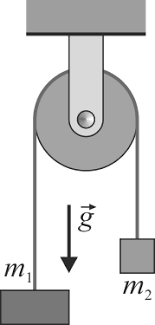
\includegraphics[scale = 0.4]{3.1_1}
\centering
\end{figure}

\noindent Si $x$ es la altura a la que se encuentra la primera masa, la altura a la que se encuentra la otra será $l-x$, donde $l$ es la longitud de la cuerda que no está pegada a la polea. Empiécese por calcular el lagrangiano del sistema. La energía cinética es
\[T = \frac{1}{2}m_1\dot{x}^2+\frac{1}{2}m_2\biggl(\frac{d}{dt}(l-x)\biggr)^2 = \frac{1}{2}(m_1+m_2)\dot{x}^2\]
y la potencial,
\[ V = -m_1gx-m_2g(l-x) = -(m_1-m_2)gx - m_2gl\]
luego
\[L = \frac{1}{2}(m_1+m_2)\dot{x}^2+(m_1-m_2)gx + m_2gl\]
El momento generalizado del sistema es
\[p = \frac{\partial L}{\partial \dot{x}} = (m_1+m_2)\dot{x}\]
Por tanto,
\[L = \frac{1}{2}\frac{p^2}{m_1+m_2} +(m_1-m_2)gx + m_2gl\]
y como las fuerzas que actúan son conservativas, se tiene que
\[H = T + V = \frac{1}{2}\frac{p^2}{m_1+m_2} -(m_1-m_2)gx - m_2gl\]
Invocando las ecuaciones canónicas,
\begin{itemize}
    \item $\displaystyle \dot{x} = \frac{p}{m_1+m_2}$
    \item $\displaystyle \dot{p} = (m_1-m_2)g \qquad$
\end{itemize}
De la primera se deduce, como ya se calculó arriba,
\[p = (m_1+m_2)\dot{x}\]
Derivando y sustituyendo en la segunda ecuación canónica, queda
\[(m_1+m_2)\ddot{x} = (m_1-m_2)g \iff \ddot{x} = \frac{m_1-m_2}{m_1+m_2}g\]
con lo que se obtiene la ecuación del movimiento del sistema.
\end{example}

\begin{example}
Se tratará de encontrar las ecuaciones de movimiento de una partícula que se mueve sobre la superficie de un cilindro de radio $R$ y que se encuentra sometida a una fuerza $\vv{F}=-k\vv{r}$, donde $r$ es la distancia al origen. La energía cinética sería
\[T = \frac{1}{2}m(\dot{x}^2+\dot{y}^2+\dot{z}^2) = \frac{1}{2}m(R^2\sen^2\theta \, \dot{\theta}^2+R^2\cos^2\theta \, \dot{\theta}^2+\dot{z}^2) = \frac{1}{2}m(R^2 \dot{\theta}^2 + \dot{z}^2)\]
y la potencial,
\[V = \frac{1}{2}kr^2 = \frac{1}{2}k(x^2+y^2+z^2) = \frac{1}{2}k(R^2+z^2)\]
de donde se obtiene el lagrangiano del sistema:
\[L = \frac{1}{2}m(R^2 \dot{\theta}^2 + \dot{z}^2)-\frac{1}{2}k(R^2+z^2)\]
En cuanto a los momentos generalizados,
\begin{itemize}
    \item $\displaystyle p_\theta = \frac{\partial L}{\partial \dot{\theta}} = mR^2\dot{\theta}$
    \item $\displaystyle p_z = \frac{\partial L}{\partial z} = m\dot{z}$
\end{itemize}
Despejando $\dot{\theta}$ y $\dot{z}$ y sustituyendo en el lagrangiano,
\[L = \frac{1}{2}m\biggl(R^2 \frac{p_\theta^2}{m^2R^4}+ \frac{p_z^2}{m^2} \biggr) - \frac{1}{2}(R^2+z^2) = \frac{p_\theta^2}{2mR^2}+\frac{p_z^2}{2m}-\frac{k(R^2+z^2)}{2}\]
Como la energía mecánica permanece constante, el hamiltoniano sería
\[H = T + V = \frac{p_\theta^2}{2mR^2}+\frac{p_z^2}{2m}+\frac{k(R^2+z^2)}{2}\]
Ahora se aplican las ecuaciones canónicas:
\begin{multicols}{2}

\begin{itemize}
    \item $\displaystyle \dot{\theta} = \frac{\partial H}{\partial p_\theta} = \frac{p_\theta}{mR^2}$
    \item $\displaystyle \dot{z} = \frac{\partial H}{\partial p_z} = \frac{p_z}{m}$
\end{itemize}

\columnbreak

\begin{itemize}
    \item $\displaystyle \dot{p}_\theta = -\frac{\partial H}{\partial \theta} = 0$
    \item $\displaystyle \dot{p}_z = -\frac{\partial H}{\partial z} = -kz$
\end{itemize}

\end{multicols}

\noindent En cuanto a los momentos generalizados, de la primera se deduce que existe una constante $k \in \R$ tal que
\[mR^2\dot{\theta} = k\]
lo que viene a decir que el momento angular se conserva. Se tiene que $p_z = m \dot{z}$, luego $\dot{p}_z = m \ddot{z}$ y por tanto
\[m\ddot{z} = -kz \iff \ddot{z} +\frac{k}{m}z = 0\]

\end{example}

\section{Transformaciones canónicas de Hamilton}

Supóngase que en un cierto problema relacionado con la mecánica hamiltoniana, las coordenadas generalizadas no resultan convenientes para resolver la cuestión. Se trata de trata de transformar el hamiltoniano $H(q_i,p_i,t)$ mediante algún truco de magia en otra función $K(Q_j,P_j,t)$ que desempeñe el mismo papel en el nuevo sistema de coordenadas. Las nuevas variables se obtendrán a partir de los anteriores, lo que se expresa como
\[Q_i = Q_i(q,p)\]
\[P_i = P_i(q,p)\]

Estaría bien que toda la monserga de las ecuaciones canónicas de Hamilton no fuese desperdiciada y pudiera usarse también en este caso. En otras palabras, se pedirá que estas funciones verifiquen
\[\frac{\partial K}{\partial P_j} = \dot{Q}_j \qquad \frac{\partial K}{\partial Q_i} = - \dot{P}_i \tag{3}\]
y cuando esto ocurra se dirá que $Q$ y $P$ son \ul{transformaciones canónicas} (recuérdese la notación $Q = (Q_1,\mathellipsis,Q_S)$, $P = (P_1,\mathellipsis,P_S)$). 

\vspace{2mm}
Con el objetivo de encontrar alguna relación entre las coordenadas antiguas $q_i, p_i$ y las nuevas $Q_i, P_i$, se va a derivar y a ver qué pasa:
\[\dot{Q} = \frac{\partial Q}{\partial q}\dot{q} + \frac{\partial Q}{\partial p}\dot{p}\]
\[\dot{P} = \frac{\partial P}{\partial q}\dot{q} + \frac{\partial P}{\partial p}\dot{p}\]
Matricialmente,
\[ \begin{pmatrix} 
    \frac{\partial Q}{\partial q} & \frac{\partial Q}{\partial p} \\[5pt]
    \frac{\partial P}{\partial q} & \frac{\partial P}{\partial p}
\end{pmatrix} \begin{pmatrix} 
    \dot{q} \\[5pt]
    \dot{p}
\end{pmatrix} = \begin{pmatrix}
    \dot{Q} \\[5pt]
    \dot{P}
\end{pmatrix} \iff MX = B\]
con lo que se podrán obtener $\dot{Q}, \dot{P}$ en función de $\dot{q}, \dot{p}$ cuando $M$ sea inversible. Es más, se verifica que las transformaciones son canónicas si y solo si $\textup{det}(M) = 1$, en cuyo caso la matriz $M$ será bautizada \ul{matriz de transformación}.

\begin{example}
Supóngase que el hamiltoniano de un cierto sistema mecánico es
\[H(q,p,t) = \frac{1}{2}p^2+\frac{1}{2}q^2\]
Aplicando las ecuaciones canónicas, se obtiene
\[q = -\dot{p} \qquad p = \dot{q} \]
Supóngase también que se tienen las funciones
\[Q(q,p) = q^2 \qquad P(q,p) = \frac{p}{2q}\]
y veamos si se tratan de transformaciones canónicas. Al expresar el hamiltoniano en términos de $P$ y $Q$, se llega a la expresión
\[H = \frac{1}{2}(\pm 2P\sqrt{Q})^2+\frac{1}{2}Q^2 = 2P^2Q+\frac{1}{2}Q^2\]
de forma que el nuevo hamiltoniano del sistema es
\[K(Q,P,t) = 2P^2Q+\frac{1}{2}Q\]
y para comprobar si se está frente a transformaciones canónicas, se calcula
\[\textup{det}(M) = \begin{vmatrix}
    2q & 0 \\[5pt]
    -\frac{p}{2q^2} & \frac{q}{2}
\end{vmatrix} = 1\]
así que las transformaciones son canónicas. Las nuevas ecuaciones canónicas serían entonces
\[4PQ = \dot{Q} \qquad 2P^2+\frac{1}{2} = -\dot{P}\]
Haciendo las cuentas que corresponden se comprueba que las dos ecuaciones anteriores se verifican, como tiene que ser.
\end{example}

\section{Funciones generadoras}

Recordando el principio de Hamilton, la trayectoria descrita en un sistema dinámico en un cierto intervalo de tiempo ha de verificar que la integral
\[S_H = \int_{t_1}^{t_2}L(q_i, \dot{q}_i,t)dt\]
sea mínima. Si esto se quiere expresar en términos de otras coordenadas $Q_i$, se tendría
\[S_K = \int_{t_1}^{t_2}L(Q_i, \dot{Q}_i,t)dt\]
Se trata entonces de encontrar alguna función que permita calcular la transformación del hamiltoniano, $K$, a partir de estas integrales. Se recuerda que el hamiltoniano del sistema no es más que
\[H(q_i,p_i,t) =\sum_{i=1}^S \dot{q}_ip_i  - L\]
y como la función $K(Q,P,t)$ verifica también las ecuaciones canónicas, entonces debería poder expresarse de la forma
\[K(Q_i,P_i,t) = \sum_{i=1}^S \dot{Q}_iP_i-L\]
Por tanto,
\[L = \sum_{i=1}^S \dot{q}_ip_i - H\]
\[L = \sum_{i=1}^S \dot{Q}_iP_i-K\]
Sustituyendo se obtiene
\[
\begin{aligned}[t]
   S_H &= \int_{t_1}^{t_2} \biggl(\sum_{i=1}^S \dot{q}_ip_i - H(q_i,\dot{p}_i,t)\biggr) dt \\
   S_K &= \int_{t_1}^{t_2} \biggl(\sum_{i=1}^S \dot{Q}_iP_i-K(Q_i,\dot{P}_i,t)\biggr) dt
\end{aligned}
\]
Que estas integrales sean mínimas significa (presupuestas ciertas condiciones de regularidad, por supuesto) que la derivada se anula. Esto se suele representar como
\[\delta S_H = 0 \qquad \delta S_K = 0\]
No merece la pena adentrarse en el significado del símbolo $\delta$; con imaginarse que es lo mismo que una derivada será más que suficiente. Se tiene entonces
\[
\begin{aligned}[t]
   \delta S_H - \delta S_K = 0 &\iff \delta (S_H - S_K) = 0 \\
   &\iff \delta \biggl( \int_{t_1}^{t_2} \biggl(\sum_{i=1}^S \dot{q}_ip_i - H\biggr) dt - \int_{t_1}^{t_2} \biggl(\sum_{i=1}^S \dot{Q}_iP_i-K dt\biggr) = 0 \\
   &\iff \delta \biggl( \int_{t_1}^{t_2} \biggl( \sum_{i=1}^S \dot{q}_ip_i - \sum_{i=1}^S \dot{Q_i}P_i +(K-H) \biggr) dt \biggr) = 0 \\
   &\overset{(*)}{\iff} \delta \biggl( \int_{t_1}^{t_2} dF_1(q_i, Q_i, t) dt \biggr) = 0
\end{aligned}
\]
Si existe una función $F_1$ que verifique $(*)$ y que dependa únicamente de $q_i, Q_i$ y $t$, se dirá que es una \ul{función generadora de tipo 1}. Nótese que una función de este estilo tiene como diferencial
\[dF_1 = \sum_{i=1}^S \frac{\partial F_1}{\partial q_i}\dot{q_i}+\sum_{i=1}^S \frac{\partial F_1}{\partial Q_i}\dot{Q_i}+\frac{\partial F_1}{\partial t}dt\]
Comparando con el integrando de la ecuación anterior, la función generadora tendrá que verificar
\[\frac{\partial F_1}{\partial q_i} = p_i \qquad \frac{\partial F_1}{\partial Q_i} = -P_i \qquad \frac{\partial F_1}{\partial t} = K-H\]
ecuaciones que resultan similares a las canónicas de Hamilton.

\vspace{2mm}
Conocida esta función generadora $F_1(q,Q,t)$, se van a obtener sin mucha justificación otras funciones generadoras $F_2(q,P,t), F_3(p,Q,t), F_4(p,P,t)$ que también cumplan $(*)$.

\begin{itemize}
    \item La función $F_2$ definida mediante 
    \[F_2(q,P,t) = F_1(q,Q,t) + QP\]
    se denomina \ul{función generadora de tipo 2}, y verifica que
    \[\frac{\partial F_2}{\partial q} = p \qquad \frac{\partial F_2}{\partial P} = Q \qquad \frac{\partial F_2}{\partial t} = K - H\]
    ya que $\frac{\partial F_1}{\partial q} = p$ y $\frac{\partial F_1}{\partial P} = 0$, pues $F_1$ no depende explícitamente de $P$.
    \item La función $F_3$ definida mediante 
    \[F_3(p,Q,t) = F_1(q,Q,t) - qp\]
    se denomina \ul{función generadora de tipo 3}, y verifica que
    \[\frac{\partial F_3}{\partial p} = - q \qquad \frac{\partial F_3}{\partial Q} = -P \qquad \frac{\partial F_3}{\partial t} = K - H\]
    ya que $\frac{\partial F_1}{\partial p} = 0$, pues $F_1$ no depende explícitamente de $p$, y $\frac{\partial F_1}{\partial Q} = -P$.
    \item La función $F_4$ definida mediante 
    \[F_4(p,P,t) = F_3(p,Q,t) + PQ\]
    se denomina \ul{función generadora de tipo 4}, y verifica que
    \[\frac{\partial F_4}{\partial p} = - q \qquad \frac{\partial F_4}{\partial P} = Q \qquad \frac{\partial F_4}{\partial t} = K - H\]
    ya que $\frac{\partial F_3}{\partial p} = -q$ y $\frac{\partial F_3}{\partial P} = 0$, pues $F_3$ no depende explícitamente de $P$.
\end{itemize}

En la práctica, cada una de estas cuatro funciones proporcionará una transformación del hamiltoniano que permita encontrar la función $K(Q,P,t)$ deseada.

\section{Ecuación de Hamilton-Jacobi}

Dado un sistema mecánico con coordenadas generalizadas $q =(q_1,\mathellipsis,q_n)$, la \ul{ecuación de Hamilton-Jacobi} es
\[\boxed{H(q,\frac{\partial S}{\partial q},t) +\frac{\partial S}{\partial t} = 0}\]
o lo que es lo mismo,
\[\boxed{H(q_1,\mathellipsis,q_S,\frac{\partial S}{\partial q_1},\mathellipsis,\frac{\partial S}{\partial q_S},t) +\frac{\partial S}{\partial t} = 0}\]
donde la solución de la ecuación $S$ es una función llamada \ul{función principal de Hamilton}. Se puede comprobar (y aquí no va a hacerse) que existen transformaciones canónicas $Q$ y $P$ de forma que $S = F_2(q,P,t)$ es una función generadora de tipo 2, y por tanto verifica
\[\frac{\partial F_2}{\partial q} = p \qquad \frac{\partial F_2}{\partial P} = Q \qquad \frac{\partial F_2}{\partial t} = K-H\]
y no solo eso, sino que en este caso se tiene que la transformación del hamiltoniano $K(Q,P,t)$ es la función nula, pues de la última expresión se deduce que
\[\frac{\partial S}{\partial t} = K - H\]
y de la ecuación de Hamilton-Jacobi,
\[\frac{\partial S}{\partial t} = - H\]
de donde se deduce que, efectivamente, $K = 0$. Esto significa, en virtud de las ecuaciones (3), que
\[\frac{\partial K}{\partial P} = \dot{Q} = 0 \qquad \frac{\partial K}{\partial Q} = - \dot{P} = 0\]
luego $Q$ y $P$ son constantes. A estas constantes se les suele denotar por $\beta = Q$ y $\alpha = P$. Total, que $S$ debe verificar
\[\boxed{\frac{\partial S}{\partial q} = p }\qquad \boxed{\frac{\partial S}{\partial \alpha} = \beta} \qquad \boxed{\frac{\partial S}{\partial t} = - H}\]

\vspace{2mm}
Un truco de magia que va a resultar de utilidad en todos los ejercicios relacionados con este asunto y que tampoco se va a justificar es suponer que la función $S$ se puede escribir como
\[\boxed{S(q,t) = \sum_{i=1}^S w_i(q_i) - \sum_{i=1}^S \alpha_it}\]
para una cierta función $w = (w_1,\mathellipsis,w_S)$. Como la variable $P = \alpha$ es constante, todo físico se puede dar el lujo de escribir $S(q,t)$ en vez de $S(q,P,t)$.

\begin{example}
Considérese un sistema mecánico conformado por una partícula de masa $m$ que se mueve en una dimensión bajo la acción de fuerzas conservativas, y cuyo hamiltoniano viene dado por
\[H(x,p,t) =\frac{p^2}{2m} + mgx\]
Se tratará de encontrar la función principal de Hamilton y una expresión para $x$. Para lo primero, supóngase que
\[S(x,t) = w(x)-\alpha t\]
Entonces se tiene que
\[\frac{\partial S}{\partial t} = -H \iff \alpha = H\]
y como las fuerzas que actúan son conservativas, el hamiltoniano coincide con la energía mecánica, de forma que $\alpha = E$ y ya solo queda encontrar $w$. Aplicando la ecuación de Hamilton-Jacobi,
\[
\begin{aligned}[t]
H(x,\frac{\partial S}{\partial x},t) + \frac{\partial S}{\partial t} = 0 &\iff \frac{1}{2m}\biggl( \frac{\partial S}{\partial x} \biggr)^2 + mgx + \frac{\partial S}{\partial t} = 0 \\
&\iff \frac{1}{2m}\biggl( \frac{\partial w}{\partial x} \biggr)^2 + mgx-E = 0 \\
&\iff \frac{\partial w}{\partial x} = \pm \sqrt{2m}\sqrt{E-mgx}
\end{aligned}
\]
suponiendo, por supuesto, que lo que hay dentro de las raíces se porta bien y no es negativo. Por tanto,
\[w(x) = \pm \sqrt{2m} \int \sqrt{E-mgx} \, dx = \mp \frac{2}{3} \frac{\sqrt{2m}}{mg}(E-mgx)^{\frac{3}{2}}\]
luego
\[S(x,t) =\mp \frac{2}{3} \frac{\sqrt{2m}}{mg}(E-mgx)^{\frac{3}{2}}-Et = \mp \frac{2\sqrt{2}}{3g\sqrt{m}}(E-mgx)^{\frac{3}{2}}-Et\]
Además, $S = w(x) - Et$ tiene que cumplir
\[
\begin{aligned}[t]
\frac{\partial S}{\partial \alpha} = \beta &\iff \frac{\partial S}{\partial E} = \beta \\[5pt]
&\iff \frac{\partial w}{\partial E} - t = \beta \\[5pt]
&\iff \pm \frac{\sqrt{2}}{g\sqrt{m}}\sqrt{E-mgx} = \beta + t \\[5pt]
&\iff \sqrt{E-mgx} = \sqrt{\frac{m}{2}}g(\beta+t) \\[5pt]
&\iff E-mgx = \frac{m}{2}g^2(\beta+t)^2 \\[5pt]
&\iff x(t)= \frac{E-\frac{m}{2}g^2(\beta+t)^2}{mg} = \frac{E}{mg} - \frac{1}{2}g(\beta+t)^2
\end{aligned}
\]

\noindent Para terminar, se intentarán hallar las constantes que se desconocen, $E$ y $\beta$. Supóngase que se conocen los datos iniciales $x_0 = x(0), v_0 = \dot{x}(0)$. Se tiene que
\[\dot{x}(t) = -g(\beta+t) \implies v_0 = \dot{x}(0) = -g\beta \implies \beta = -\frac{v_0}{g}\]
luego
\[x(t) = \frac{E}{mg} - \frac{1}{2}g\biggl(-\frac{v_0}{g}+t\biggr)^2 = \frac{E}{mg} - \frac{1}{2}g\biggl(\frac{v_0^2}{g^2}+t^2-\frac{2v_0t}{g}\biggr)\]
Poniendo $t = 0$,
\[x_0 = \frac{E}{mg} -\frac{1}{2}\frac{v_0^2}{g} \implies E = mgx_0+\frac{1}{2}mv_0^2\]
Conclusión:
\[x(t) = x_0+\frac{1}{2}\frac{v_0^2}{g}-\frac{1}{2}\frac{v_0^2}{g}-\frac{1}{2}gt^2+v_0t = x_0+v_0t-\frac{1}{2}gt^2\]
y el problema en cuestión no era más que una caída libre.
\end{example}

\chapter{Teoría especial de la relatividad}

\section{Transformación de Galileo}

Sean $K$, $K'$ dos sistemas de referencia inerciales (es decir, que uno respecto del otro está en reposo o se mueve a velocidad constante) y supongamos que ambos se mueven a una velocidad constante $v$ en la dirección de sus ejes $x_1$ y $x_1'$.

\begin{figure}[h]
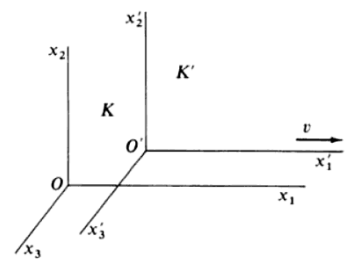
\includegraphics[scale = 0.75]{4.1_1}
\centering
\end{figure}

Según la mecánica de Newton, el tiempo es una magnitud absoluta e independiente del sistema de referencia. Si se llama $t$ al tiempo medido por un observador en el sistema de referencia $K$ y $t'$ al tiempo medido por otro observador en $K'$, se tendrá que $t = t'$. Además, si se denota por  $(x_1,x_2,x_3)$ y $(x_1', x_2',x_3')$ a la posición de una partícula respecto de cada uno de los sistemas, entonces se tendrán las relaciones
\[
\left\{
\begin{aligned}
    x_1' &=x_1-vt \\
    x_2' &=x_2 \\
    x_3' &=x_3 \\
    t    &=t'
\end{aligned}
\right.
\]
Estas ecuaciones se dice que definen una \ul{transformación de Galileo}.

\vspace{2mm}
En consecuencia, si un haz de luz se mueve desde el sistema $K$ hacia el $K'$ con velocidades $c$ y $c'$ respecto de cada uno de los sistemas, según la primera ecuación de la transformación de Galileo, estas velocidades estarán relacionadas por
\[c' = c - v\]
y esto contradice las \textit{leyes de Maxwell}, según las cuales la velocidad de la luz en el vacío es una constante absoluta y universal, independiente de todo movimiento relativo entre fuente y observador. 

\vspace{2mm}
En esta discrepancia, observaciones experimentales dan la razón a la invarianza de la velocidad de la luz respecto de sistemas de referencias distintos.

\begin{example}
Considérense los dos sistemas de referencia $K$, $K'$ de antes, ahora suponiendo que el primero no se mueve y que se ubica un tren sobre el eje $x_1'$ de $K'$. 

\vspace{2mm}
\noindent Supóngase que un rayo de luz sale del suelo del tren y rebota con el techo, que se encuentra a una altura $h$. El tiempo que tardará el rayo en regresar al punto de salida será
\[t' = \frac{2h}{c}\]
donde $c$ es la constante universal de la velocidad de la luz. 

\vspace{2mm}
\noindent Ahora se calculará este mismo tiempo desde el punto de vista de un observador que se encuentre sobre el sistema $K$. Para este individuo, el rayo de luz no solo se mueve en el eje $x_2$, sino que también lo hace en el $x_1$. 

\vspace{2mm}
\noindent Llámese $A$ a la posición en el eje $x_1$ del rayo en el instante inicial, $B$ a la del instante en que toca el techo, y $C$ a la del instante final. Por simetría, el tiempo que tarda el rayo en subir y bajar es el doble del tiempo que tarda en subir. Por tanto,
\[t = \frac{2}{c}\sqrt{(B-A)^2+h^2}\]
 Aquí convendría hacer un esquema del panorama que ilustre la expresión anterior. También se tiene que
\[t = \frac{2(B-A)}{v} \iff B-A = \frac{vt}{2}\]
Sustituyendo y despejando,
\[t = \frac{2}{c}\sqrt{\frac{v^2t^2}{4}+h^2} \iff  c^2t^2 = v^2t^2+4h^2 \iff t = \frac{2h}{\sqrt{c^2-v^2}} = t' \, \frac{1}{\sqrt{1-\frac{v^2}{c^2}}}\]
lo que relaciona el tiempo desde el punto de vista de cada uno de los sistemas de referencia. 

\vspace{2mm}
\noindent Si se examina la longitud del tren según cada sistema de referencia, también se hallarán resultados curiosos. Para ello, el observador del sistema $K$ se situaría delante del tren, mediría el tiempo $\Delta t$ que tarda en pasar frente a él, y afirmaría que la longitud del tren es
\[L = v \, \Delta t\]
Simultáneamente, el observador del sistema $K'$ ha medido un tiempo $\Delta t'$. La longitud del tren entonces será
\[L' = v \, \Delta t'\]
Hay que tener en cuenta que antes el observador de $K'$ que medía el tiempo se encontraba en reposo, y el de $K$ estaba en movimiento subido en el tren (se recuerda que el sistema de referencia $K$ no se mueve y el $K'$ lo hace a velocidad constante). Ahora se tiene que el observador de $K$ está en reposo y el de $K'$ en movimiento, pues ambos están midiendo el tiempo desde fuera del tren. Entonces
\[\Delta t' = \frac{2h}{\sqrt{c^2-v^2}} = \Delta t \, \frac{1}{\sqrt{1-\frac{v^2}{c^2}}}\]
luego
\[L' = \frac{1}{\sqrt{1-\frac{v^2}{c^2}}} \, L\]
lo que quiere decir que el tren es más corto desde el punto de vista del observador de $K'$.
\end{example}

En general, a una diferencia en el tiempo trancurrido medido por dos observadores se le llama \ul{dilatación del tiempo}. De la cantidad
\[\gamma = \frac{1}{\sqrt{1-\frac{v^2}{c^2}}}\]
se dirá que es el \ul{índice de Lorentz}.

\section{Transformación de Lorentz}

Ya se ha visto en la sección anterior que la transformación de Galileo va a servir de poco si se quieren respetar las leyes de Maxwell, así que habrá que apañárselas de otra forma para encontrar una relación entre las coordenadas de los sistemas de referencia $K$ y $K'$ que tenga en cuenta la invarianza de la velocidad de la luz.

\vspace{2mm}
Que el tiempo no sea absoluto y común a todos los sistemas de referencia afecta al asunto de las coordenadas, pues este se comporta como una coordenada más. Para que no haya ninguna trifulca entre unidades de posición y unidades de tiempo, la coordenada del tiempo se expresará muchas veces en la forma $ct$.

\vspace{2mm}
Dados dos sistemas de referencia $K$ y $K'$ tales que uno se mueve respecto del otro a velocidad constante $v$ en la dirección del eje $x$, a las ecuaciones
\[
\left\{
\begin{aligned}
    x' &= \gamma(x-vt) \\
    y' &= y \\
    z' &= z \\
    t' &= \gamma(t-\frac{v}{c^2}x)
\end{aligned}
\right.
\]
que relacionan las coordenadas de $K$ y $K'$, se les conoce como \ul{transformación de Lorentz}. La transformación inversa sería
\[
\left\{
\begin{aligned}
    x &= \gamma(x'+vt') \\
    y &= y' \\
    z &= z' \\
    t &= \gamma(t'+\frac{v}{c^2}x')
\end{aligned}
\right.
\]


\vspace{2mm}
Sin entrar en detalle, estas transformaciones concuerdan con el comportamiento de la velocidad de la luz en sistemas de referencia cualesquiera que se encuentren en las condiciones antes mencionadas.

\vspace{2mm}
Una vez resuelto el problema de encontrar las relaciones entre la posición de una partícula en cada uno de los sistemas, habrá que examinar qué pasa con las velocidades. 

\vspace{2mm}
Si tiene lugar una pequeña variación en las coordenadas de la partícula (lo que se denotará por $dx'$ y $dx$ en el caso de la primera coordenada, por ejemplo), según las ecuaciones de la transformación de Lorentz,
\[dx' = \gamma (dx - v \, dt)\]
\[dt' = \gamma (dt - \frac{v}{c^2} \, dx)\]
por lo que la velocidad en el eje $x$ de $K'$ sería
\[v'_x = \frac{dx'}{dt'} = \frac{dx-v \, dt}{dt - \frac{v}{c^2} \, dx} = \frac{\frac{dx}{dt} - v}{1 - \frac{v}{c^2}\frac{dx}{dt}} = \frac{v_x - v}{1-\frac{v}{c^2} \, v_x}\]
y en el eje $y$,
\[v_y' = \frac{dy'}{dt'} = \frac{dy}{\gamma(dt-\frac{v}{c^2} \, dx)} = \frac{\frac{dy}{dt}}{\gamma(1-\frac{v}{c^2}\frac{dx}{dt})} = \frac{v_y}{\gamma (1-\frac{v}{c^2}v_x)}\]
y en el eje $z$,
\[v_z' =  \frac{v_z}{\gamma (1-\frac{v}{c^2}v_x)}\]
En resumidas cuentas,
\[
\left\{
\begin{aligned}
    v_x' &= \frac{v_x-v}{1-\frac{v}{c^2}v_x} \\[5pt]
    v_y' &= \frac{v_y}{\gamma(1-\frac{v}{c^2}v_x)} \\[5pt]
    v_z' &= \frac{v_z}{\gamma(1-\frac{v}{c^2}v_x)}
\end{aligned}
\right.
\]

\section{Formulación de Minkowski}

Hermann Minkowski sugería que el tiempo se tenía que considerar como otra coordenada sobre la cual la transformación de Lorentz actúa como una rotación. Partiendo de las ecuaciones de Lorentz, se tiene
\[
\left\{
\begin{aligned}
    ct' &= \gamma(ct-\frac{v}{c} \, x_2) \\
    x_2' &= \gamma(x_2-\frac{v}{c} \, ct) \\
    x_3' &= x_3 \\
    x_4' &= x_4 \\
\end{aligned}
\right.
\]
donde el tiempo ha sido multiplicado por $c$ y el resto de coordenadas han sido renombradas. Lo de multiplicar y dividir por $c$ en la segunda ecuación tendrá su utilidad a continuación. Llamando $x_1' = ct'$, $x_1 = ct$ y $\beta = \frac{v}{c}$, puede escribirse
\[
\left\{
\begin{aligned}
    x_1' &= \gamma x_1-\beta \gamma x_2 \\
    x_2' &= \gamma x_2-\beta \gamma x_1 \\
    x_3' &= x_3 \\
    x_4' &= x_4 \\
\end{aligned}
\right.
\]
Matricialmente,
\[
\begin{pmatrix}
    x_1' \\
    x_2' \\
    x_3' \\
    x_4'
\end{pmatrix} = \begin{pmatrix}
    \gamma & -\beta \gamma & 0 & 0 \\
    -\beta \gamma & \gamma  & 0 & 0 \\
    0 & 0 & 1 & 0 \\
    0 & 0 & 0 & 1
\end{pmatrix} \begin{pmatrix*}[r]
    x_1 \\
    x_2 \\
    x_3 \\
    x_4
\end{pmatrix*}
\]

\vspace{2mm}
A continuación se razonará qué tiene que ver todo esto con la rotación que se mencionó principio de la sección. Tómese un ángulo $\phi$ tal que $\gamma = \textup{cosh} \, \phi$. Se tiene entonces
\[\textup{cosh} \, \phi = \frac{1}{\sqrt{1-\beta^2}} \implies \textup{cosh}^2 \, \phi = \frac{1}{1-\beta^2}\]
y como bien es sabido que $\textup{cosh}^2 \, \phi - \textup{senh}^2 \, \phi = 1$, entonces
\[1+\textup{senh}^2 \, \phi = \frac{1}{1-\beta^2} \iff \textup{senh}^2 \, \phi = \frac{1-1+\beta^2}{1-\beta^2} = \gamma^2 \beta^2\]
luego $\textup{sinh} \, \phi = \gamma \beta$ y la ecuación matricial anterior quedaría
\[
\begin{pmatrix}
    x_1' \\
    x_2' \\
    x_3' \\
    x_4'
\end{pmatrix} = \begin{pmatrix}
    \phantom{-}\textup{cosh} \, \phi & -\textup{senh} \, \phi & 0 & 0 \\
    -\textup{senh} \, \phi & \phantom{-}\textup{cosh} \, \phi & 0 & 0 \\
    \phantom{-}0 & \phantom{-}0 & 1 & 0 \\
    \phantom{-}0 & \phantom{-}0 & 0 & 1
\end{pmatrix} \begin{pmatrix*}[r]
    x_1 \\
    x_2 \\
    x_3 \\
    x_4
\end{pmatrix*}
\]
de forma que la matriz cuadrada se asemeja de sobremanera a una matriz de rotación en $\R^4$. Además, unas simples cuentas demuestran que
\[(x_1')^2-(x_2')^2 = x_1^2-x_2^2\]
y por tanto,
\[(x_1')^2-(x_2')^2-(x_3')^2-(x_4')^2 = x_1^2-x_2^2-x_3^2-x_4^2\]
o, equivalentemente, cambiando al gusto el nombre de las coordenadas,
\[(ct')^2-(x')^2-(y')^2-(z')^2 = (ct)^2-x^2-y^2-z^2\]
expresión cuya finalidad será desvelada en breve.

\section{Cuadrivectores}

La notación que se usará ahora a partir de ahora para las cuatro coordenadas en un cierto sistema de referencia será 
\[(x^0, x^1, x^2, x^3) \equiv (ct, x, y, z)\]
donde en la primera coordenada a veces se escribe directamente el tiempo $t$ en lugar de $ct$. Estos vectores de $\R^4$ se denominan \ul{cuadrivectores}. Los cuadrivectores son elementos del llamado \ul{espacio-tiempo de Minkowski}. En ocasiones se denotará
\[\mathbb{X}^u \equiv (x^0,x^1,x^2,x^3)\]
o incluso
\[\mathbb{X}^u \equiv (x^0, x^i)\]
con objeto de separar la coordenada correspondiente al tiempo del resto.

\vspace{2mm}
De la misma forma que en el espacio euclídeo había un elemento de distancia para medir el desplazamiento de un vector, el análogo en el espacio de Minkowski será la cantidad $ds$ tal que
\[ds^2 = (dx^0)^2 - (dx^1)^2 - (dx^2)^2 - (dx^3)^2\]
la cual se ha visto antes que permanece constante ante cambios en el sistema de referencia. 

\vspace{2mm}
Prosiguiendo con las analogías, al igual que en el espacio euclídeo se definen producto escalar y norma euclídeos a partir de la distancia, en el espacio de Minkowski, dados dos cuadrivectores $\mathbb{A}^u = (a^0,a^1,a^2,a^3)$ y $\mathbb{B}^u = (b^0,b^1,b^2,b^3)$, su \ul{producto escalar} será
\[\mathbb{A}^u \cdot \mathbb{B}^u = a^0b^0 - a^1b^1-a^2b^2-a^3b^3\]
mientras que la \ul{norma},
\[||\mathbb{A}^u|| = \sqrt{(x^0)^2-(x^1)^2-(x^2)^2-(x^3)^2}\]

\vspace{2mm}
Es una auténtica lástima que los términos \textit{cuadriproducto escalar} y \textit{cuadrinorma} estén en desuso, con lo natural que resulta enchufarle el prefijo \textit{cuadri} a todo lo que tenga que ver con cuadrivectores.

\vspace{2mm}
Otra invariante con cierta relevancia en el espacio-tiempo de Minkowski es el \ul{tiempo propio}, magnitud definida como
\[d\tau = dt \sqrt{1 - \frac{v^2}{c^2}}\]
En efecto, se tiene que
\[d\tau = dt \, \sqrt{1 - \frac{1}{c^2}\biggl(\frac{dx^2}{dt^2}+\frac{dy^2}{dt^2}+\frac{dz^2}{dt^2}\biggr)} = \sqrt{dt^2 - \frac{1}{c^2}(x^2+y^2+z^2)} = \sqrt{\frac{ds^2}{c^2}} = \frac{ds}{c}\]
donde $ds$, $c$ son constantes. 

\vspace{2mm}
Dado un desplazamiento $(dx^0,dx^1,dx^2,dx^3)$ de un cuadrivector $(x^0,x^1,x^2,x^3)$, se define su \ul{cuadrivelocidad} como
\[\mathbb{U}^u \equiv (u^0, u^1, u^2, u^3) = \biggl( \frac{dx^0}{d\tau}, \frac{dx^1}{d\tau}, \frac{dx^2}{d\tau}, \frac{dx^3}{d\tau} \biggr)\]
En analogía con la notación de los cuadrivectores, también se escribe
\[\mathbb{U}^u = (u^0, u^i)\]
A partir de la expresión del tiempo propio se obtiene
\[ u^0 = \frac{c\, dt}{dt \, \sqrt{1-\frac{v^2}{c^2}}} = \frac{c}{\sqrt{1-\frac{v^2}{c^2}}} \qquad \qquad  u^i = \frac{dx^i}{dt \, \sqrt{1-\frac{v^2}{c^2}}} = \frac{v^i}{\sqrt{1-\frac{v^2}{c^2}}}\]
luego
\[\boxed{\mathbb{U}^u = (\gamma c,\gamma v^i)}\]
Se comprueba inmediatamente que
\[\gamma^2 c^2 - \gamma^2 (v^i)^2 = c^2\]
es decir,
\[\boxed{||\mathbb{U}^u||^2 = c^2}\]
\section{Lagrangiano relativista y hamiltoniano relativista}

Dada una partícula que sigue una cierta trayectoria en el espacio y sobre la que no actúan fuerzas externas, se recuerda que el punto de partida de la mecánica lagrangiana era encontrar una cierta cantidad escalar $S$ que se hacía mínima a lo largo de dicha trayectoria. Razonamientos físicos que no van a ser expuestos obligan a que $S$ sea de la forma
\[S = \int_B^A -mc^2 \, d\tau\]
De acuerdo con la definición de tiempo propio,
\[S = \int_B^A -mc^2 \, \sqrt{1-\frac{v^2}{c^2}} \, dt\]
Por tanto, el \ul{lagrangiano relativista} de la partícula se define como
\[\boxed{\underset{\phantom{\sum}}{L}  = -mc^2 \sqrt{1-\frac{v^2}{c^2}}}\]

\vspace{2mm}
La siguiente misión es hallar el hamiltoniano. Los \ul{momentos generalizados relativistas}, de forma natural, se definen como
\[p^i = \frac{\partial L}{\partial \dot{x}^i}\]
o lo que es lo mismo, teniendo en cuenta que puede escribirse $v = (\dot{x}^1)^2 + (\dot{x}^2)^2+(\dot{x}^3)^2$,
\[p^i = mc^2 \frac{\frac{\dot{x}^i}{c^2}}{\sqrt{1-\frac{v^2}{c^2}}} = \frac{m\dot{x}^i}{\sqrt{1-\frac{v^2}{c^2}}} = mu^i\]
y también puede escribirse
\[p^0 = mu^0\]
Los momentos generalizados relativistas se denotarán como
\[\mathbb{P}^u \equiv m\mathbb{U}^u\]
o bien
\[\mathbb{P}^u \equiv (p^0, p^i)\]
Ya se está en condiciones de encontrar el hamiltoniano:
\[H = \sum_{i=0}^3 p^i \dot{x}^i - L = \sum_{i=0}^3 \frac{m(\dot{x}^i)^2}{\sqrt{1-\frac{v^2}{c^2}}} - L = \frac{mv^2}{\sqrt{1-\frac{v^2}{c^2}}} + mc^2 \sqrt{1-\frac{v^2}{c^2}} = \frac{mv^2+mc^2(1-\frac{v^2}{c^2})}{\sqrt{1-\frac{v^2}{c^2}}}\]
Por tanto, el \ul{hamiltoniano relativista} se define como
\[\boxed{H = \frac{mc^2}{\sqrt{1-v^2/c^2}}}\]

En ausencia de fuerzas externas, el hamiltoniano relativista coincide con la energía mecánica. Supóngase que la partícula está en reposo $(v = 0)$ y lo que ocurrirá entonces es histórico:

\begin{center}
    \fcolorbox{black}{MediumPurple}{$E = mc^2$}
\end{center}

Ni más ni menos que la célebre ecuación de Einstein. Se colorea de morado el recuadro en homenaje a este famoso científico, pues, según cuentan las leyendas urbanas, era éste el color de su frondoso bigote. Como todas las imágenes suyas que existen están blanco y negro, nadie puede atreverse a desmentir semejante verdad.

\vspace{2mm}
En caso de que solo actúen fuerzas conservativas (y por tanto $H = E$), resulta más o menos intuitivo definir la \ul{energía cinética relativista} como la diferencia entre la energía mecánica y la energía en reposo:
\[\boxed{T = (\gamma-1)mc^2}\]

\vspace{2mm}
Por otro lado, se recuerda que la expresión de la primera componente de la cuadrivelocidad era
\[u^0 = \frac{c}{\sqrt{1-\frac{v^2}{c^2}}}\]
luego
\[p^0 = mu^0 = \frac{mc}{\sqrt{1-\frac{v^2}{c^2}}} = \frac{E}{c}\]
Respecto a las otras componentes,
\[p^i = mu^i = \frac{mv^i}{\sqrt{1-\frac{v^2}{c^2}}} = \gamma mv^i\]
así que el momento espacial no es más que
\[\boxed{\mathbb{P}^u = \biggl(\frac{E}{c}, \gamma m v^1, \gamma m v^2,  \gamma m v^3 \biggr)}\]

\vspace{2mm}
Por último, se van a demostrar algunas expresiones útiles en relación con la energía y el momento. Veamos que
\[\boxed{E^2 = (pc)^2+(mc^2)^2}\]
donde $E$ es la energía total, $m$ es la masa del cuerpo cuando está en reposo y $p$ es el vector de $\R^3$ formado por las coordenadas espaciales del momento relativista, es decir, \[p = \gamma m_0 v = (\gamma m_0 v^1, \gamma m_0 v^2, \gamma m_0 v^3) = (p^1,p^2,p^3)\]
Se tiene que
\[p^2 = p \cdot p = \gamma^2 m^2 (v \cdot v) = \gamma^2 m^2 v^2 = \frac{m^2v^2}{1-\frac{v^2}{c^2}}\]
Despejando $v^2$ se obtiene
\[v^2 = \frac{p^2c^2}{m^2c^2+p^2}\]
luego
\[\gamma = \frac{1}{\sqrt{1-\frac{p^2}{p^2+m^2c^2}}} = \sqrt{\frac{p^2+m^2c^2}{m^2c^2}} = \sqrt{1+\biggl(\frac{p}{mc}\biggr)^2}\]
Por tanto,
\[E = \gamma m c^2 = mc^2\sqrt{1+\biggl(\frac{p}{mc}\biggr)^2}\]
y al elevar al cuadrado se obtiene la expresión buscada. Por último, también se verifica que
\[\boxed{||\mathbb{P}^u||^2 = m^2c^2}\]
lo cual se deduce de
\[\frac{E^2}{c^2}-\gamma^2m^2(v^1)^2-\gamma^2m^2(v^2)^2-\gamma^2m^2(v^3)^2 = m^2c^2\]
\end{document}
